\documentclass[twoside]{book}

% Packages required by doxygen
\usepackage{calc}
\usepackage{doxygen}
\usepackage{graphicx}
\usepackage[utf8]{inputenc}
\usepackage{makeidx}
\usepackage{multicol}
\usepackage{multirow}
\usepackage{textcomp}
\usepackage[table]{xcolor}

% Font selection
\usepackage[T1]{fontenc}
\usepackage{mathptmx}
\usepackage[scaled=.90]{helvet}
\usepackage{courier}
\usepackage{amssymb}
\usepackage{sectsty}
\renewcommand{\familydefault}{\sfdefault}
\allsectionsfont{%
  \fontseries{bc}\selectfont%
  \color{darkgray}%
}
\renewcommand{\DoxyLabelFont}{%
  \fontseries{bc}\selectfont%
  \color{darkgray}%
}

% Page & text layout
\usepackage{geometry}
\geometry{%
  a4paper,%
  top=2.5cm,%
  bottom=2.5cm,%
  left=2.5cm,%
  right=2.5cm%
}
\tolerance=750
\hfuzz=15pt
\hbadness=750
\setlength{\emergencystretch}{15pt}
\setlength{\parindent}{0cm}
\setlength{\parskip}{0.2cm}
\makeatletter
\renewcommand{\paragraph}{%
  \@startsection{paragraph}{4}{0ex}{-1.0ex}{1.0ex}{%
    \normalfont\normalsize\bfseries\SS@parafont%
  }%
}
\renewcommand{\subparagraph}{%
  \@startsection{subparagraph}{5}{0ex}{-1.0ex}{1.0ex}{%
    \normalfont\normalsize\bfseries\SS@subparafont%
  }%
}
\makeatother

% Headers & footers
\usepackage{fancyhdr}
\pagestyle{fancyplain}
\fancyhead[LE]{\fancyplain{}{\bfseries\thepage}}
\fancyhead[CE]{\fancyplain{}{}}
\fancyhead[RE]{\fancyplain{}{\bfseries\leftmark}}
\fancyhead[LO]{\fancyplain{}{\bfseries\rightmark}}
\fancyhead[CO]{\fancyplain{}{}}
\fancyhead[RO]{\fancyplain{}{\bfseries\thepage}}
\fancyfoot[LE]{\fancyplain{}{}}
\fancyfoot[CE]{\fancyplain{}{}}
\fancyfoot[RE]{\fancyplain{}{\bfseries\scriptsize Generated on Fri Feb 23 2018 15\-:32\-:14 for Class Scheduler by Doxygen }}
\fancyfoot[LO]{\fancyplain{}{\bfseries\scriptsize Generated on Fri Feb 23 2018 15\-:32\-:14 for Class Scheduler by Doxygen }}
\fancyfoot[CO]{\fancyplain{}{}}
\fancyfoot[RO]{\fancyplain{}{}}
\renewcommand{\footrulewidth}{0.4pt}
\renewcommand{\chaptermark}[1]{%
  \markboth{#1}{}%
}
\renewcommand{\sectionmark}[1]{%
  \markright{\thesection\ #1}%
}

% Indices & bibliography
\usepackage{natbib}
\usepackage[titles]{tocloft}
\setcounter{tocdepth}{3}
\setcounter{secnumdepth}{5}
\makeindex

% Hyperlinks (required, but should be loaded last)
\usepackage{ifpdf}
\ifpdf
  \usepackage[pdftex,pagebackref=true]{hyperref}
\else
  \usepackage[ps2pdf,pagebackref=true]{hyperref}
\fi
\hypersetup{%
  colorlinks=true,%
  linkcolor=blue,%
  citecolor=blue,%
  unicode%
}

% Custom commands
\newcommand{\clearemptydoublepage}{%
  \newpage{\pagestyle{empty}\cleardoublepage}%
}


%===== C O N T E N T S =====

\begin{document}

% Titlepage & ToC
\hypersetup{pageanchor=false}
\pagenumbering{roman}
\begin{titlepage}
\vspace*{7cm}
\begin{center}%
{\Large Class Scheduler \\[1ex]\large 0.\-0.\-1 }\\
\vspace*{1cm}
{\large Generated by Doxygen 1.8.6}\\
\vspace*{0.5cm}
{\small Fri Feb 23 2018 15:32:14}\\
\end{center}
\end{titlepage}
\clearemptydoublepage
\tableofcontents
\clearemptydoublepage
\pagenumbering{arabic}
\hypersetup{pageanchor=true}

%--- Begin generated contents ---
\chapter{Namespace Index}
\section{Namespace List}
Here is a list of all documented namespaces with brief descriptions\-:\begin{DoxyCompactList}
\item\contentsline{section}{\hyperlink{namespaceimport__faculty__data}{import\-\_\-faculty\-\_\-data} }{\pageref{namespaceimport__faculty__data}}{}
\item\contentsline{section}{\hyperlink{namespaceimport__room__data}{import\-\_\-room\-\_\-data} }{\pageref{namespaceimport__room__data}}{}
\item\contentsline{section}{\hyperlink{namespacemysite_1_1settings}{mysite.\-settings} }{\pageref{namespacemysite_1_1settings}}{}
\item\contentsline{section}{\hyperlink{namespacemysite_1_1urls}{mysite.\-urls} }{\pageref{namespacemysite_1_1urls}}{}
\item\contentsline{section}{\hyperlink{namespacemysite_1_1wsgi}{mysite.\-wsgi} }{\pageref{namespacemysite_1_1wsgi}}{}
\item\contentsline{section}{\hyperlink{namespacesettings}{settings} }{\pageref{namespacesettings}}{}
\end{DoxyCompactList}

\chapter{Hierarchical Index}
\section{Class Hierarchy}
This inheritance list is sorted roughly, but not completely, alphabetically\-:\begin{DoxyCompactList}
\item Base\-Consideration\begin{DoxyCompactList}
\item \contentsline{section}{osd.\-considerations.\-Base\-Constraint}{\pageref{interfaceosd_1_1considerations_1_1_base_constraint}}{}
\item \contentsline{section}{osd.\-considerations.\-Base\-Preference}{\pageref{interfaceosd_1_1considerations_1_1_base_preference}}{}
\end{DoxyCompactList}
\item \contentsline{section}{osd.\-considerations.\-Base\-Consideration\-Module}{\pageref{classosd_1_1considerations_1_1_base_consideration_module}}{}
\item \contentsline{section}{osd.\-database.\-Block\-Record}{\pageref{classosd_1_1database_1_1_block_record}}{}
\item \contentsline{section}{osd.\-input.\-Block\-Set}{\pageref{classosd_1_1input_1_1_block_set}}{}
\item \contentsline{section}{osd.\-output.\-Callbacks}{\pageref{interfaceosd_1_1output_1_1_callbacks}}{}
\item \contentsline{section}{osd.\-considerations.\-Consideration$<$ Boolean $>$}{\pageref{interfaceosd_1_1considerations_1_1_consideration}}{}
\begin{DoxyCompactList}
\item \contentsline{section}{osd.\-considerations.\-Constraint}{\pageref{interfaceosd_1_1considerations_1_1_constraint}}{}
\begin{DoxyCompactList}
\item \contentsline{section}{osd.\-considerations.\-Constraint.\-Blacklist}{\pageref{interfaceosd_1_1considerations_1_1_constraint_1_1_blacklist}}{}
\item \contentsline{section}{osd.\-considerations.\-Constraint.\-Whitelist}{\pageref{interfaceosd_1_1considerations_1_1_constraint_1_1_whitelist}}{}
\item \contentsline{section}{osd.\-considerations.\-User\-Constraint}{\pageref{classosd_1_1considerations_1_1_user_constraint}}{}
\end{DoxyCompactList}
\end{DoxyCompactList}
\item \contentsline{section}{osd.\-considerations.\-Consideration$<$ Integer $>$}{\pageref{interfaceosd_1_1considerations_1_1_consideration}}{}
\begin{DoxyCompactList}
\item \contentsline{section}{osd.\-considerations.\-Preference}{\pageref{interfaceosd_1_1considerations_1_1_preference}}{}
\begin{DoxyCompactList}
\item \contentsline{section}{osd.\-considerations.\-User\-Preference}{\pageref{classosd_1_1considerations_1_1_user_preference}}{}
\end{DoxyCompactList}
\end{DoxyCompactList}
\item \contentsline{section}{osd.\-database.\-Course\-Record}{\pageref{classosd_1_1database_1_1_course_record}}{}
\item Database\-Factory\begin{DoxyCompactList}
\item \contentsline{section}{osd.\-database.\-Block\-Factory}{\pageref{classosd_1_1database_1_1_block_factory}}{}
\item \contentsline{section}{osd.\-database.\-Course\-Factory}{\pageref{classosd_1_1database_1_1_course_factory}}{}
\item \contentsline{section}{osd.\-database.\-Professor\-Factory}{\pageref{classosd_1_1database_1_1_professor_factory}}{}
\item \contentsline{section}{osd.\-database.\-Room\-Factory}{\pageref{classosd_1_1database_1_1_room_factory}}{}
\item \contentsline{section}{osd.\-database.\-User\-Constraint\-Factory}{\pageref{classosd_1_1database_1_1_user_constraint_factory}}{}
\item \contentsline{section}{osd.\-database.\-User\-Preference\-Factory}{\pageref{classosd_1_1database_1_1_user_preference_factory}}{}
\item \contentsline{section}{osd.\-input.\-Professor\-Factory}{\pageref{classosd_1_1input_1_1_professor_factory}}{}
\end{DoxyCompactList}
\item \contentsline{section}{osd.\-database.\-Database\-Module}{\pageref{classosd_1_1database_1_1_database_module}}{}
\item \contentsline{section}{osd.\-main.\-Flag\-Module}{\pageref{classosd_1_1main_1_1_flag_module}}{}
\item \contentsline{section}{osd.\-main.\-Flags}{\pageref{classosd_1_1main_1_1_flags}}{}
\item \contentsline{section}{osd.\-input.\-placeholder.\-Placeholder.\-From\-C\-S\-V}{\pageref{interfaceosd_1_1input_1_1placeholder_1_1_placeholder_1_1_from_c_s_v}}{}
\item \contentsline{section}{osd.\-output.\-Hunk}{\pageref{classosd_1_1output_1_1_hunk}}{}
\item \contentsline{section}{osd.\-input.\-Input\-Module}{\pageref{classosd_1_1input_1_1_input_module}}{}
\item \contentsline{section}{osd.\-considerations.\-Lookups}{\pageref{interfaceosd_1_1considerations_1_1_lookups}}{}
\item \contentsline{section}{scheduler.\-models.\-Named.\-Meta}{\pageref{classscheduler_1_1models_1_1_named_1_1_meta}}{}
\item \contentsline{section}{scheduler.\-models.\-User\-Preference\-Or\-Constraint.\-Meta}{\pageref{classscheduler_1_1models_1_1_user_preference_or_constraint_1_1_meta}}{}
\item Migration\begin{DoxyCompactList}
\item \contentsline{section}{faculty\-\_\-data.\-migrations.0001\-\_\-initial.Migration}{\pageref{classfaculty__data_1_1migrations_1_10001__initial_1_1_migration}}{}
\item \contentsline{section}{room\-\_\-data.\-migrations.0001\-\_\-initial.Migration}{\pageref{classroom__data_1_1migrations_1_10001__initial_1_1_migration}}{}
\item \contentsline{section}{room\-\_\-data.\-migrations.0002\-\_\-auto\-\_\-20180226\-\_\-1350.Migration}{\pageref{classroom__data_1_1migrations_1_10002__auto__20180226__1350_1_1_migration}}{}
\end{DoxyCompactList}
\item Model\begin{DoxyCompactList}
\item \contentsline{section}{faculty\-\_\-data.\-models.\-Faculty}{\pageref{classfaculty__data_1_1models_1_1_faculty}}{}
\item \contentsline{section}{room\-\_\-data.\-models.\-Room}{\pageref{classroom__data_1_1models_1_1_room}}{}
\item \contentsline{section}{scheduler.\-models.\-Hunk}{\pageref{classscheduler_1_1models_1_1_hunk}}{}
\item \contentsline{section}{scheduler.\-models.\-Named}{\pageref{classscheduler_1_1models_1_1_named}}{}
\begin{DoxyCompactList}
\item \contentsline{section}{scheduler.\-models.\-Block}{\pageref{classscheduler_1_1models_1_1_block}}{}
\item \contentsline{section}{scheduler.\-models.\-Course}{\pageref{classscheduler_1_1models_1_1_course}}{}
\item \contentsline{section}{scheduler.\-models.\-Division}{\pageref{classscheduler_1_1models_1_1_division}}{}
\item \contentsline{section}{scheduler.\-models.\-Professor}{\pageref{classscheduler_1_1models_1_1_professor}}{}
\item \contentsline{section}{scheduler.\-models.\-Room\-Type}{\pageref{classscheduler_1_1models_1_1_room_type}}{}
\end{DoxyCompactList}
\item \contentsline{section}{scheduler.\-models.\-Pregen\-Section}{\pageref{classscheduler_1_1models_1_1_pregen_section}}{}
\item \contentsline{section}{scheduler.\-models.\-Room}{\pageref{classscheduler_1_1models_1_1_room}}{}
\item \contentsline{section}{scheduler.\-models.\-Section}{\pageref{classscheduler_1_1models_1_1_section}}{}
\item \contentsline{section}{scheduler.\-models.\-User\-Preference\-Or\-Constraint}{\pageref{classscheduler_1_1models_1_1_user_preference_or_constraint}}{}
\begin{DoxyCompactList}
\item \contentsline{section}{scheduler.\-models.\-User\-Constraint}{\pageref{classscheduler_1_1models_1_1_user_constraint}}{}
\item \contentsline{section}{scheduler.\-models.\-User\-Preference}{\pageref{classscheduler_1_1models_1_1_user_preference}}{}
\end{DoxyCompactList}
\end{DoxyCompactList}
\item \contentsline{section}{osd.\-input.\-Named}{\pageref{interfaceosd_1_1input_1_1_named}}{}
\begin{DoxyCompactList}
\item \contentsline{section}{osd.\-input.\-Block}{\pageref{interfaceosd_1_1input_1_1_block}}{}
\item \contentsline{section}{osd.\-input.\-Course}{\pageref{interfaceosd_1_1input_1_1_course}}{}
\item \contentsline{section}{osd.\-input.\-Professor}{\pageref{interfaceosd_1_1input_1_1_professor}}{}
\item \contentsline{section}{osd.\-input.\-Room}{\pageref{interfaceosd_1_1input_1_1_room}}{}
\item \contentsline{section}{osd.\-input.\-Room\-Type}{\pageref{interfaceosd_1_1input_1_1_room_type}}{}
\item \contentsline{section}{osd.\-input.\-Section}{\pageref{interfaceosd_1_1input_1_1_section}}{}
\end{DoxyCompactList}
\item \contentsline{section}{scheduler.\-csv\-\_\-parser.\-Parse\-Mode}{\pageref{classscheduler_1_1csv__parser_1_1_parse_mode}}{}
\begin{DoxyCompactList}
\item \contentsline{section}{scheduler.\-csv\-\_\-parser.\-Block\-Parser}{\pageref{classscheduler_1_1csv__parser_1_1_block_parser}}{}
\item \contentsline{section}{scheduler.\-csv\-\_\-parser.\-Room\-Parser}{\pageref{classscheduler_1_1csv__parser_1_1_room_parser}}{}
\end{DoxyCompactList}
\item \contentsline{section}{osd.\-input.\-placeholder.\-Placeholder\-Module}{\pageref{classosd_1_1input_1_1placeholder_1_1_placeholder_module}}{}
\item \contentsline{section}{osd.\-database.\-Professor\-Record}{\pageref{classosd_1_1database_1_1_professor_record}}{}
\item Relation\begin{DoxyCompactList}
\item \contentsline{section}{osd.\-util.\-relation.\-Many\-To\-Many\-Relation$<$ K, V $>$}{\pageref{classosd_1_1util_1_1relation_1_1_many_to_many_relation_3_01_k_00_01_v_01_4}}{}
\item \contentsline{section}{osd.\-util.\-relation.\-Many\-To\-One\-Relation$<$ K, V $>$}{\pageref{classosd_1_1util_1_1relation_1_1_many_to_one_relation_3_01_k_00_01_v_01_4}}{}
\item \contentsline{section}{osd.\-util.\-relation.\-One\-To\-Many\-Relation$<$ K, V $>$}{\pageref{classosd_1_1util_1_1relation_1_1_one_to_many_relation_3_01_k_00_01_v_01_4}}{}
\end{DoxyCompactList}
\item \contentsline{section}{osd.\-util.\-relation.\-Relation$<$ K, L, V, W $>$}{\pageref{classosd_1_1util_1_1relation_1_1_relation_3_01_k_00_01_l_00_01_v_00_01_w_01_4}}{}
\item \contentsline{section}{osd.\-output.\-Results}{\pageref{interfaceosd_1_1output_1_1_results}}{}
\item \contentsline{section}{osd.\-database.\-Room\-Record}{\pageref{classosd_1_1database_1_1_room_record}}{}
\item \contentsline{section}{hibernate1.\-Run\-Tables}{\pageref{classhibernate1_1_1_run_tables}}{}
\item \contentsline{section}{osd.\-schedule.\-Schedule\-Module}{\pageref{interfaceosd_1_1schedule_1_1_schedule_module}}{}
\item \contentsline{section}{osd.\-schedule.\-Scheduler}{\pageref{interfaceosd_1_1schedule_1_1_scheduler}}{}
\item \contentsline{section}{osd.\-main.\-Scheduling}{\pageref{interfaceosd_1_1main_1_1_scheduling}}{}
\item \contentsline{section}{osd.\-input.\-Sources}{\pageref{interfaceosd_1_1input_1_1_sources}}{}
\item \contentsline{section}{osd.\-input.\-Input\-Module.\-Sources\-Module}{\pageref{interfaceosd_1_1input_1_1_input_module_1_1_sources_module}}{}
\item \contentsline{section}{osd.\-considerations.\-User\-Consideration\-Module}{\pageref{classosd_1_1considerations_1_1_user_consideration_module}}{}
\item \contentsline{section}{osd.\-database.\-User\-Constraint\-Record}{\pageref{classosd_1_1database_1_1_user_constraint_record}}{}
\item \contentsline{section}{osd.\-database.\-User\-Preference\-Record}{\pageref{classosd_1_1database_1_1_user_preference_record}}{}
\item App\-Config\begin{DoxyCompactList}
\item \contentsline{section}{faculty\-\_\-data.\-apps.\-Faculty\-Data\-Config}{\pageref{classfaculty__data_1_1apps_1_1_faculty_data_config}}{}
\item \contentsline{section}{polls.\-apps.\-Polls\-Config}{\pageref{classpolls_1_1apps_1_1_polls_config}}{}
\item \contentsline{section}{room\-\_\-data.\-apps.\-Room\-Data\-Config}{\pageref{classroom__data_1_1apps_1_1_room_data_config}}{}
\item \contentsline{section}{scheduler.\-apps.\-Scheduler\-Config}{\pageref{classscheduler_1_1apps_1_1_scheduler_config}}{}
\end{DoxyCompactList}
\item Base\-Command\begin{DoxyCompactList}
\item \contentsline{section}{import\-\_\-faculty\-\_\-data.\-Command}{\pageref{classimport__faculty__data_1_1_command}}{}
\item \contentsline{section}{import\-\_\-room\-\_\-data.\-Command}{\pageref{classimport__room__data_1_1_command}}{}
\end{DoxyCompactList}
\item Function\begin{DoxyCompactList}
\item \contentsline{section}{osd.\-considerations.\-Consideration$<$ T $>$}{\pageref{interfaceosd_1_1considerations_1_1_consideration_3_01_t_01_4}}{}
\end{DoxyCompactList}
\item Predicate\begin{DoxyCompactList}
\item \contentsline{section}{osd.\-considerations.\-Consideration}{\pageref{interfaceosd_1_1considerations_1_1_consideration}}{}
\begin{DoxyCompactList}
\item \contentsline{section}{osd.\-considerations.\-Constraint}{\pageref{interfaceosd_1_1considerations_1_1_constraint}}{}
\item \contentsline{section}{osd.\-considerations.\-Preference}{\pageref{interfaceosd_1_1considerations_1_1_preference}}{}
\item \contentsline{section}{osd.\-considerations.\-User\-Consideration}{\pageref{classosd_1_1considerations_1_1_user_consideration}}{}
\begin{DoxyCompactList}
\item \contentsline{section}{osd.\-considerations.\-User\-Constraint}{\pageref{classosd_1_1considerations_1_1_user_constraint}}{}
\item \contentsline{section}{osd.\-considerations.\-User\-Preference}{\pageref{classosd_1_1considerations_1_1_user_preference}}{}
\end{DoxyCompactList}
\end{DoxyCompactList}
\item \contentsline{section}{osd.\-considerations.\-Constraint}{\pageref{interfaceosd_1_1considerations_1_1_constraint}}{}
\end{DoxyCompactList}
\item Serializable\begin{DoxyCompactList}
\item \contentsline{section}{hibernate1.\-Test\-Table}{\pageref{classhibernate1_1_1_test_table}}{}
\end{DoxyCompactList}
\item Test\-Case\begin{DoxyCompactList}
\item \contentsline{section}{scheduler.\-tests.\-Test\-Models}{\pageref{classscheduler_1_1tests_1_1_test_models}}{}
\end{DoxyCompactList}
\end{DoxyCompactList}

\chapter{Class Index}
\section{Class List}
Here are the classes, structs, unions and interfaces with brief descriptions\-:\begin{DoxyCompactList}
\item\contentsline{section}{\hyperlink{classosd_1_1considerations_1_1_base_consideration_module}{osd.\-considerations.\-Base\-Consideration\-Module} }{\pageref{classosd_1_1considerations_1_1_base_consideration_module}}{}
\item\contentsline{section}{\hyperlink{interfaceosd_1_1considerations_1_1_base_constraint}{osd.\-considerations.\-Base\-Constraint} }{\pageref{interfaceosd_1_1considerations_1_1_base_constraint}}{}
\item\contentsline{section}{\hyperlink{interfaceosd_1_1considerations_1_1_base_preference}{osd.\-considerations.\-Base\-Preference} }{\pageref{interfaceosd_1_1considerations_1_1_base_preference}}{}
\item\contentsline{section}{\hyperlink{interfaceosd_1_1considerations_1_1_constraint_1_1_blacklist}{osd.\-considerations.\-Constraint.\-Blacklist} }{\pageref{interfaceosd_1_1considerations_1_1_constraint_1_1_blacklist}}{}
\item\contentsline{section}{\hyperlink{classscheduler_1_1models_1_1_block}{scheduler.\-models.\-Block} }{\pageref{classscheduler_1_1models_1_1_block}}{}
\item\contentsline{section}{\hyperlink{interfaceosd_1_1input_1_1_block}{osd.\-input.\-Block} }{\pageref{interfaceosd_1_1input_1_1_block}}{}
\item\contentsline{section}{\hyperlink{classosd_1_1database_1_1_block_factory}{osd.\-database.\-Block\-Factory} }{\pageref{classosd_1_1database_1_1_block_factory}}{}
\item\contentsline{section}{\hyperlink{classscheduler_1_1csv__parser_1_1_block_parser}{scheduler.\-csv\-\_\-parser.\-Block\-Parser} }{\pageref{classscheduler_1_1csv__parser_1_1_block_parser}}{}
\item\contentsline{section}{\hyperlink{classosd_1_1database_1_1_block_record}{osd.\-database.\-Block\-Record} }{\pageref{classosd_1_1database_1_1_block_record}}{}
\item\contentsline{section}{\hyperlink{classosd_1_1input_1_1_block_set}{osd.\-input.\-Block\-Set} }{\pageref{classosd_1_1input_1_1_block_set}}{}
\item\contentsline{section}{\hyperlink{interfaceosd_1_1output_1_1_callbacks}{osd.\-output.\-Callbacks} }{\pageref{interfaceosd_1_1output_1_1_callbacks}}{}
\item\contentsline{section}{\hyperlink{classimport__faculty__data_1_1_command}{import\-\_\-faculty\-\_\-data.\-Command} }{\pageref{classimport__faculty__data_1_1_command}}{}
\item\contentsline{section}{\hyperlink{classimport__room__data_1_1_command}{import\-\_\-room\-\_\-data.\-Command} }{\pageref{classimport__room__data_1_1_command}}{}
\item\contentsline{section}{\hyperlink{interfaceosd_1_1considerations_1_1_consideration}{osd.\-considerations.\-Consideration} }{\pageref{interfaceosd_1_1considerations_1_1_consideration}}{}
\item\contentsline{section}{\hyperlink{interfaceosd_1_1considerations_1_1_consideration_3_01_t_01_4}{osd.\-considerations.\-Consideration$<$ T $>$} }{\pageref{interfaceosd_1_1considerations_1_1_consideration_3_01_t_01_4}}{}
\item\contentsline{section}{\hyperlink{interfaceosd_1_1considerations_1_1_constraint}{osd.\-considerations.\-Constraint} }{\pageref{interfaceosd_1_1considerations_1_1_constraint}}{}
\item\contentsline{section}{\hyperlink{interfaceosd_1_1input_1_1_course}{osd.\-input.\-Course} }{\pageref{interfaceosd_1_1input_1_1_course}}{}
\item\contentsline{section}{\hyperlink{classscheduler_1_1models_1_1_course}{scheduler.\-models.\-Course} }{\pageref{classscheduler_1_1models_1_1_course}}{}
\item\contentsline{section}{\hyperlink{classosd_1_1database_1_1_course_factory}{osd.\-database.\-Course\-Factory} }{\pageref{classosd_1_1database_1_1_course_factory}}{}
\item\contentsline{section}{\hyperlink{classosd_1_1database_1_1_course_record}{osd.\-database.\-Course\-Record} }{\pageref{classosd_1_1database_1_1_course_record}}{}
\item\contentsline{section}{\hyperlink{classosd_1_1database_1_1_database_module}{osd.\-database.\-Database\-Module} }{\pageref{classosd_1_1database_1_1_database_module}}{}
\item\contentsline{section}{\hyperlink{classscheduler_1_1models_1_1_division}{scheduler.\-models.\-Division} }{\pageref{classscheduler_1_1models_1_1_division}}{}
\item\contentsline{section}{\hyperlink{classfaculty__data_1_1models_1_1_faculty}{faculty\-\_\-data.\-models.\-Faculty} }{\pageref{classfaculty__data_1_1models_1_1_faculty}}{}
\item\contentsline{section}{\hyperlink{classfaculty__data_1_1apps_1_1_faculty_data_config}{faculty\-\_\-data.\-apps.\-Faculty\-Data\-Config} }{\pageref{classfaculty__data_1_1apps_1_1_faculty_data_config}}{}
\item\contentsline{section}{\hyperlink{classosd_1_1main_1_1_flag_module}{osd.\-main.\-Flag\-Module} }{\pageref{classosd_1_1main_1_1_flag_module}}{}
\item\contentsline{section}{\hyperlink{classosd_1_1main_1_1_flags}{osd.\-main.\-Flags} }{\pageref{classosd_1_1main_1_1_flags}}{}
\item\contentsline{section}{\hyperlink{interfaceosd_1_1input_1_1placeholder_1_1_placeholder_1_1_from_c_s_v}{osd.\-input.\-placeholder.\-Placeholder.\-From\-C\-S\-V} }{\pageref{interfaceosd_1_1input_1_1placeholder_1_1_placeholder_1_1_from_c_s_v}}{}
\item\contentsline{section}{\hyperlink{classosd_1_1output_1_1_hunk}{osd.\-output.\-Hunk} }{\pageref{classosd_1_1output_1_1_hunk}}{}
\item\contentsline{section}{\hyperlink{classscheduler_1_1models_1_1_hunk}{scheduler.\-models.\-Hunk} }{\pageref{classscheduler_1_1models_1_1_hunk}}{}
\item\contentsline{section}{\hyperlink{classosd_1_1input_1_1_input_module}{osd.\-input.\-Input\-Module} }{\pageref{classosd_1_1input_1_1_input_module}}{}
\item\contentsline{section}{\hyperlink{interfaceosd_1_1considerations_1_1_lookups}{osd.\-considerations.\-Lookups} }{\pageref{interfaceosd_1_1considerations_1_1_lookups}}{}
\item\contentsline{section}{\hyperlink{classosd_1_1util_1_1relation_1_1_many_to_many_relation_3_01_k_00_01_v_01_4}{osd.\-util.\-relation.\-Many\-To\-Many\-Relation$<$ K, V $>$} }{\pageref{classosd_1_1util_1_1relation_1_1_many_to_many_relation_3_01_k_00_01_v_01_4}}{}
\item\contentsline{section}{\hyperlink{classosd_1_1util_1_1relation_1_1_many_to_one_relation_3_01_k_00_01_v_01_4}{osd.\-util.\-relation.\-Many\-To\-One\-Relation$<$ K, V $>$} }{\pageref{classosd_1_1util_1_1relation_1_1_many_to_one_relation_3_01_k_00_01_v_01_4}}{}
\item\contentsline{section}{\hyperlink{classscheduler_1_1models_1_1_named_1_1_meta}{scheduler.\-models.\-Named.\-Meta} }{\pageref{classscheduler_1_1models_1_1_named_1_1_meta}}{}
\item\contentsline{section}{\hyperlink{classscheduler_1_1models_1_1_user_preference_or_constraint_1_1_meta}{scheduler.\-models.\-User\-Preference\-Or\-Constraint.\-Meta} }{\pageref{classscheduler_1_1models_1_1_user_preference_or_constraint_1_1_meta}}{}
\item\contentsline{section}{\hyperlink{classfaculty__data_1_1migrations_1_10001__initial_1_1_migration}{faculty\-\_\-data.\-migrations.\-0001\-\_\-initial.\-Migration} }{\pageref{classfaculty__data_1_1migrations_1_10001__initial_1_1_migration}}{}
\item\contentsline{section}{\hyperlink{classroom__data_1_1migrations_1_10001__initial_1_1_migration}{room\-\_\-data.\-migrations.\-0001\-\_\-initial.\-Migration} }{\pageref{classroom__data_1_1migrations_1_10001__initial_1_1_migration}}{}
\item\contentsline{section}{\hyperlink{classroom__data_1_1migrations_1_10002__auto__20180226__1350_1_1_migration}{room\-\_\-data.\-migrations.\-0002\-\_\-auto\-\_\-20180226\-\_\-1350.\-Migration} }{\pageref{classroom__data_1_1migrations_1_10002__auto__20180226__1350_1_1_migration}}{}
\item\contentsline{section}{\hyperlink{interfaceosd_1_1input_1_1_named}{osd.\-input.\-Named} }{\pageref{interfaceosd_1_1input_1_1_named}}{}
\item\contentsline{section}{\hyperlink{classscheduler_1_1models_1_1_named}{scheduler.\-models.\-Named} }{\pageref{classscheduler_1_1models_1_1_named}}{}
\item\contentsline{section}{\hyperlink{classosd_1_1util_1_1relation_1_1_one_to_many_relation_3_01_k_00_01_v_01_4}{osd.\-util.\-relation.\-One\-To\-Many\-Relation$<$ K, V $>$} }{\pageref{classosd_1_1util_1_1relation_1_1_one_to_many_relation_3_01_k_00_01_v_01_4}}{}
\item\contentsline{section}{\hyperlink{classscheduler_1_1csv__parser_1_1_parse_mode}{scheduler.\-csv\-\_\-parser.\-Parse\-Mode} }{\pageref{classscheduler_1_1csv__parser_1_1_parse_mode}}{}
\item\contentsline{section}{\hyperlink{classosd_1_1input_1_1placeholder_1_1_placeholder_module}{osd.\-input.\-placeholder.\-Placeholder\-Module} }{\pageref{classosd_1_1input_1_1placeholder_1_1_placeholder_module}}{}
\item\contentsline{section}{\hyperlink{classpolls_1_1apps_1_1_polls_config}{polls.\-apps.\-Polls\-Config} }{\pageref{classpolls_1_1apps_1_1_polls_config}}{}
\item\contentsline{section}{\hyperlink{interfaceosd_1_1considerations_1_1_preference}{osd.\-considerations.\-Preference} }{\pageref{interfaceosd_1_1considerations_1_1_preference}}{}
\item\contentsline{section}{\hyperlink{classscheduler_1_1models_1_1_pregen_section}{scheduler.\-models.\-Pregen\-Section} }{\pageref{classscheduler_1_1models_1_1_pregen_section}}{}
\item\contentsline{section}{\hyperlink{interfaceosd_1_1input_1_1_professor}{osd.\-input.\-Professor} }{\pageref{interfaceosd_1_1input_1_1_professor}}{}
\item\contentsline{section}{\hyperlink{classscheduler_1_1models_1_1_professor}{scheduler.\-models.\-Professor} }{\pageref{classscheduler_1_1models_1_1_professor}}{}
\item\contentsline{section}{\hyperlink{classosd_1_1input_1_1_professor_factory}{osd.\-input.\-Professor\-Factory} }{\pageref{classosd_1_1input_1_1_professor_factory}}{}
\item\contentsline{section}{\hyperlink{classosd_1_1database_1_1_professor_factory}{osd.\-database.\-Professor\-Factory} }{\pageref{classosd_1_1database_1_1_professor_factory}}{}
\item\contentsline{section}{\hyperlink{classosd_1_1database_1_1_professor_record}{osd.\-database.\-Professor\-Record} }{\pageref{classosd_1_1database_1_1_professor_record}}{}
\item\contentsline{section}{\hyperlink{classosd_1_1util_1_1relation_1_1_relation_3_01_k_00_01_l_00_01_v_00_01_w_01_4}{osd.\-util.\-relation.\-Relation$<$ K, L, V, W $>$} }{\pageref{classosd_1_1util_1_1relation_1_1_relation_3_01_k_00_01_l_00_01_v_00_01_w_01_4}}{}
\item\contentsline{section}{\hyperlink{interfaceosd_1_1output_1_1_results}{osd.\-output.\-Results} }{\pageref{interfaceosd_1_1output_1_1_results}}{}
\item\contentsline{section}{\hyperlink{interfaceosd_1_1input_1_1_room}{osd.\-input.\-Room} }{\pageref{interfaceosd_1_1input_1_1_room}}{}
\item\contentsline{section}{\hyperlink{classroom__data_1_1models_1_1_room}{room\-\_\-data.\-models.\-Room} }{\pageref{classroom__data_1_1models_1_1_room}}{}
\item\contentsline{section}{\hyperlink{classscheduler_1_1models_1_1_room}{scheduler.\-models.\-Room} }{\pageref{classscheduler_1_1models_1_1_room}}{}
\item\contentsline{section}{\hyperlink{classroom__data_1_1apps_1_1_room_data_config}{room\-\_\-data.\-apps.\-Room\-Data\-Config} }{\pageref{classroom__data_1_1apps_1_1_room_data_config}}{}
\item\contentsline{section}{\hyperlink{classosd_1_1database_1_1_room_factory}{osd.\-database.\-Room\-Factory} }{\pageref{classosd_1_1database_1_1_room_factory}}{}
\item\contentsline{section}{\hyperlink{classscheduler_1_1csv__parser_1_1_room_parser}{scheduler.\-csv\-\_\-parser.\-Room\-Parser} }{\pageref{classscheduler_1_1csv__parser_1_1_room_parser}}{}
\item\contentsline{section}{\hyperlink{classosd_1_1database_1_1_room_record}{osd.\-database.\-Room\-Record} }{\pageref{classosd_1_1database_1_1_room_record}}{}
\item\contentsline{section}{\hyperlink{interfaceosd_1_1input_1_1_room_type}{osd.\-input.\-Room\-Type} }{\pageref{interfaceosd_1_1input_1_1_room_type}}{}
\item\contentsline{section}{\hyperlink{classscheduler_1_1models_1_1_room_type}{scheduler.\-models.\-Room\-Type} }{\pageref{classscheduler_1_1models_1_1_room_type}}{}
\item\contentsline{section}{\hyperlink{classhibernate1_1_1_run_tables}{hibernate1.\-Run\-Tables} }{\pageref{classhibernate1_1_1_run_tables}}{}
\item\contentsline{section}{\hyperlink{interfaceosd_1_1schedule_1_1_schedule_module}{osd.\-schedule.\-Schedule\-Module} }{\pageref{interfaceosd_1_1schedule_1_1_schedule_module}}{}
\item\contentsline{section}{\hyperlink{interfaceosd_1_1schedule_1_1_scheduler}{osd.\-schedule.\-Scheduler} }{\pageref{interfaceosd_1_1schedule_1_1_scheduler}}{}
\item\contentsline{section}{\hyperlink{classscheduler_1_1apps_1_1_scheduler_config}{scheduler.\-apps.\-Scheduler\-Config} }{\pageref{classscheduler_1_1apps_1_1_scheduler_config}}{}
\item\contentsline{section}{\hyperlink{interfaceosd_1_1main_1_1_scheduling}{osd.\-main.\-Scheduling} }{\pageref{interfaceosd_1_1main_1_1_scheduling}}{}
\item\contentsline{section}{\hyperlink{classscheduler_1_1models_1_1_section}{scheduler.\-models.\-Section} }{\pageref{classscheduler_1_1models_1_1_section}}{}
\item\contentsline{section}{\hyperlink{interfaceosd_1_1input_1_1_section}{osd.\-input.\-Section} }{\pageref{interfaceosd_1_1input_1_1_section}}{}
\item\contentsline{section}{\hyperlink{interfaceosd_1_1input_1_1_sources}{osd.\-input.\-Sources} }{\pageref{interfaceosd_1_1input_1_1_sources}}{}
\item\contentsline{section}{\hyperlink{interfaceosd_1_1input_1_1_input_module_1_1_sources_module}{osd.\-input.\-Input\-Module.\-Sources\-Module} }{\pageref{interfaceosd_1_1input_1_1_input_module_1_1_sources_module}}{}
\item\contentsline{section}{\hyperlink{classscheduler_1_1tests_1_1_test_models}{scheduler.\-tests.\-Test\-Models} }{\pageref{classscheduler_1_1tests_1_1_test_models}}{}
\item\contentsline{section}{\hyperlink{classhibernate1_1_1_test_table}{hibernate1.\-Test\-Table} }{\pageref{classhibernate1_1_1_test_table}}{}
\item\contentsline{section}{\hyperlink{classosd_1_1considerations_1_1_user_consideration}{osd.\-considerations.\-User\-Consideration} }{\pageref{classosd_1_1considerations_1_1_user_consideration}}{}
\item\contentsline{section}{\hyperlink{classosd_1_1considerations_1_1_user_consideration_module}{osd.\-considerations.\-User\-Consideration\-Module} }{\pageref{classosd_1_1considerations_1_1_user_consideration_module}}{}
\item\contentsline{section}{\hyperlink{classosd_1_1considerations_1_1_user_constraint}{osd.\-considerations.\-User\-Constraint} }{\pageref{classosd_1_1considerations_1_1_user_constraint}}{}
\item\contentsline{section}{\hyperlink{classscheduler_1_1models_1_1_user_constraint}{scheduler.\-models.\-User\-Constraint} }{\pageref{classscheduler_1_1models_1_1_user_constraint}}{}
\item\contentsline{section}{\hyperlink{classosd_1_1database_1_1_user_constraint_factory}{osd.\-database.\-User\-Constraint\-Factory} }{\pageref{classosd_1_1database_1_1_user_constraint_factory}}{}
\item\contentsline{section}{\hyperlink{classosd_1_1database_1_1_user_constraint_record}{osd.\-database.\-User\-Constraint\-Record} }{\pageref{classosd_1_1database_1_1_user_constraint_record}}{}
\item\contentsline{section}{\hyperlink{classosd_1_1considerations_1_1_user_preference}{osd.\-considerations.\-User\-Preference} }{\pageref{classosd_1_1considerations_1_1_user_preference}}{}
\item\contentsline{section}{\hyperlink{classscheduler_1_1models_1_1_user_preference}{scheduler.\-models.\-User\-Preference} }{\pageref{classscheduler_1_1models_1_1_user_preference}}{}
\item\contentsline{section}{\hyperlink{classosd_1_1database_1_1_user_preference_factory}{osd.\-database.\-User\-Preference\-Factory} }{\pageref{classosd_1_1database_1_1_user_preference_factory}}{}
\item\contentsline{section}{\hyperlink{classscheduler_1_1models_1_1_user_preference_or_constraint}{scheduler.\-models.\-User\-Preference\-Or\-Constraint} }{\pageref{classscheduler_1_1models_1_1_user_preference_or_constraint}}{}
\item\contentsline{section}{\hyperlink{classosd_1_1database_1_1_user_preference_record}{osd.\-database.\-User\-Preference\-Record} }{\pageref{classosd_1_1database_1_1_user_preference_record}}{}
\item\contentsline{section}{\hyperlink{interfaceosd_1_1considerations_1_1_constraint_1_1_whitelist}{osd.\-considerations.\-Constraint.\-Whitelist} }{\pageref{interfaceosd_1_1considerations_1_1_constraint_1_1_whitelist}}{}
\end{DoxyCompactList}

\chapter{Namespace Documentation}
\hypertarget{namespacemysite_1_1settings}{\section{mysite.\-settings Namespace Reference}
\label{namespacemysite_1_1settings}\index{mysite.\-settings@{mysite.\-settings}}
}
\subsection*{Variables}
\begin{DoxyCompactItemize}
\item 
\hypertarget{namespacemysite_1_1settings_addb5cd2f2982b7eb7113b40cdfdf0e7d}{tuple {\bfseries B\-A\-S\-E\-\_\-\-D\-I\-R} = os.\-path.\-dirname(os.\-path.\-dirname(os.\-path.\-abspath(\-\_\-\-\_\-file\-\_\-\-\_\-)))}\label{namespacemysite_1_1settings_addb5cd2f2982b7eb7113b40cdfdf0e7d}

\item 
\hypertarget{namespacemysite_1_1settings_ab2aed82d2734b39d5387b22b7a953de5}{string {\bfseries S\-E\-C\-R\-E\-T\-\_\-\-K\-E\-Y} = 'f\#sa$^\wedge$zkf(p3)uyu9t1d6hbq1fuc\%$\ast$u\&5ojlpk22\#\-\_\-6gu0pzirg'}\label{namespacemysite_1_1settings_ab2aed82d2734b39d5387b22b7a953de5}

\item 
\hypertarget{namespacemysite_1_1settings_ae7ae0ac83176d533cc1c1d84862c82bf}{{\bfseries D\-E\-B\-U\-G} = True}\label{namespacemysite_1_1settings_ae7ae0ac83176d533cc1c1d84862c82bf}

\item 
\hypertarget{namespacemysite_1_1settings_ab6f4415a608815b8ca5f84d320437cf8}{list {\bfseries A\-L\-L\-O\-W\-E\-D\-\_\-\-H\-O\-S\-T\-S} = \mbox{[}'192.\-168.\-1.\-38', '127.\-0.\-0.\-1', '172.\-19.\-3.\-99', 'localhost'\mbox{]}}\label{namespacemysite_1_1settings_ab6f4415a608815b8ca5f84d320437cf8}

\item 
\hypertarget{namespacemysite_1_1settings_a626f4fd3c8256437791205c2ce7b0cdd}{string {\bfseries L\-O\-G\-I\-N\-\_\-\-R\-E\-D\-I\-R\-E\-C\-T\-\_\-\-U\-R\-L} = 'home'}\label{namespacemysite_1_1settings_a626f4fd3c8256437791205c2ce7b0cdd}

\item 
list {\bfseries I\-N\-S\-T\-A\-L\-L\-E\-D\-\_\-\-A\-P\-P\-S}
\item 
list {\bfseries M\-I\-D\-D\-L\-E\-W\-A\-R\-E}
\item 
\hypertarget{namespacemysite_1_1settings_ab0a7fa8cdaaccbf5bf874db67cbe507a}{string {\bfseries R\-O\-O\-T\-\_\-\-U\-R\-L\-C\-O\-N\-F} = 'mysite.\-urls'}\label{namespacemysite_1_1settings_ab0a7fa8cdaaccbf5bf874db67cbe507a}

\item 
list {\bfseries T\-E\-M\-P\-L\-A\-T\-E\-S}
\item 
\hypertarget{namespacemysite_1_1settings_a7e476bde6438ad8065a7d9f5b4a759ba}{string {\bfseries W\-S\-G\-I\-\_\-\-A\-P\-P\-L\-I\-C\-A\-T\-I\-O\-N} = 'mysite.\-wsgi.\-application'}\label{namespacemysite_1_1settings_a7e476bde6438ad8065a7d9f5b4a759ba}

\item 
dictionary {\bfseries D\-A\-T\-A\-B\-A\-S\-E\-S}
\item 
list {\bfseries A\-U\-T\-H\-\_\-\-P\-A\-S\-S\-W\-O\-R\-D\-\_\-\-V\-A\-L\-I\-D\-A\-T\-O\-R\-S}
\item 
\hypertarget{namespacemysite_1_1settings_a5aa2d89c65baaf7b41e64a82ed412029}{string {\bfseries L\-A\-N\-G\-U\-A\-G\-E\-\_\-\-C\-O\-D\-E} = 'en-\/us'}\label{namespacemysite_1_1settings_a5aa2d89c65baaf7b41e64a82ed412029}

\item 
\hypertarget{namespacemysite_1_1settings_a8166ffe52ad58ff798949b613c9b5b2c}{string {\bfseries T\-I\-M\-E\-\_\-\-Z\-O\-N\-E} = 'U\-T\-C'}\label{namespacemysite_1_1settings_a8166ffe52ad58ff798949b613c9b5b2c}

\item 
\hypertarget{namespacemysite_1_1settings_af3b43f8f116e73ded7f3ce336e7499ac}{{\bfseries U\-S\-E\-\_\-\-I18\-N} = True}\label{namespacemysite_1_1settings_af3b43f8f116e73ded7f3ce336e7499ac}

\item 
\hypertarget{namespacemysite_1_1settings_abaf7e237dddf19bbdecee0f0167c2e06}{{\bfseries U\-S\-E\-\_\-\-L10\-N} = True}\label{namespacemysite_1_1settings_abaf7e237dddf19bbdecee0f0167c2e06}

\item 
\hypertarget{namespacemysite_1_1settings_a58cd46ff574d992b401f49fd371e0b24}{{\bfseries U\-S\-E\-\_\-\-T\-Z} = True}\label{namespacemysite_1_1settings_a58cd46ff574d992b401f49fd371e0b24}

\item 
\hypertarget{namespacemysite_1_1settings_a2aa5b2f0ed54dd3f8965ca2786f7fc27}{string {\bfseries S\-T\-A\-T\-I\-C\-\_\-\-U\-R\-L} = '/static/'}\label{namespacemysite_1_1settings_a2aa5b2f0ed54dd3f8965ca2786f7fc27}

\end{DoxyCompactItemize}


\subsection{Detailed Description}
\begin{DoxyVerb}Django settings for mysite project.

Generated by 'django-admin startproject' using Django 2.0.2.

For more information on this file, see
https://docs.djangoproject.com/en/2.0/topics/settings/

For the full list of settings and their values, see
https://docs.djangoproject.com/en/2.0/ref/settings/
\end{DoxyVerb}
 

\subsection{Variable Documentation}
\hypertarget{namespacemysite_1_1settings_ae1a1bb374bc9383cde47414d4aaa23bc}{\index{mysite\-::settings@{mysite\-::settings}!A\-U\-T\-H\-\_\-\-P\-A\-S\-S\-W\-O\-R\-D\-\_\-\-V\-A\-L\-I\-D\-A\-T\-O\-R\-S@{A\-U\-T\-H\-\_\-\-P\-A\-S\-S\-W\-O\-R\-D\-\_\-\-V\-A\-L\-I\-D\-A\-T\-O\-R\-S}}
\index{A\-U\-T\-H\-\_\-\-P\-A\-S\-S\-W\-O\-R\-D\-\_\-\-V\-A\-L\-I\-D\-A\-T\-O\-R\-S@{A\-U\-T\-H\-\_\-\-P\-A\-S\-S\-W\-O\-R\-D\-\_\-\-V\-A\-L\-I\-D\-A\-T\-O\-R\-S}!mysite::settings@{mysite\-::settings}}
\subsubsection[{A\-U\-T\-H\-\_\-\-P\-A\-S\-S\-W\-O\-R\-D\-\_\-\-V\-A\-L\-I\-D\-A\-T\-O\-R\-S}]{\setlength{\rightskip}{0pt plus 5cm}list mysite.\-settings.\-A\-U\-T\-H\-\_\-\-P\-A\-S\-S\-W\-O\-R\-D\-\_\-\-V\-A\-L\-I\-D\-A\-T\-O\-R\-S}}\label{namespacemysite_1_1settings_ae1a1bb374bc9383cde47414d4aaa23bc}
{\bfseries Initial value\-:}
\begin{DoxyCode}
1 = [
2     \{
3         \textcolor{stringliteral}{'NAME'}: \textcolor{stringliteral}{'django.contrib.auth.password\_validation.UserAttributeSimilarityValidator'},
4     \},
5     \{
6         \textcolor{stringliteral}{'NAME'}: \textcolor{stringliteral}{'django.contrib.auth.password\_validation.MinimumLengthValidator'},
7     \},
8     \{
9         \textcolor{stringliteral}{'NAME'}: \textcolor{stringliteral}{'django.contrib.auth.password\_validation.CommonPasswordValidator'},
10     \},
11     \{
12         \textcolor{stringliteral}{'NAME'}: \textcolor{stringliteral}{'django.contrib.auth.password\_validation.NumericPasswordValidator'},
13     \},
14 ]
\end{DoxyCode}
\hypertarget{namespacemysite_1_1settings_a04300628acd12c08ea63ee5f9d3d83d1}{\index{mysite\-::settings@{mysite\-::settings}!D\-A\-T\-A\-B\-A\-S\-E\-S@{D\-A\-T\-A\-B\-A\-S\-E\-S}}
\index{D\-A\-T\-A\-B\-A\-S\-E\-S@{D\-A\-T\-A\-B\-A\-S\-E\-S}!mysite::settings@{mysite\-::settings}}
\subsubsection[{D\-A\-T\-A\-B\-A\-S\-E\-S}]{\setlength{\rightskip}{0pt plus 5cm}dictionary mysite.\-settings.\-D\-A\-T\-A\-B\-A\-S\-E\-S}}\label{namespacemysite_1_1settings_a04300628acd12c08ea63ee5f9d3d83d1}
{\bfseries Initial value\-:}
\begin{DoxyCode}
1 = \{
2     \textcolor{stringliteral}{'default'}: \{
3         \textcolor{stringliteral}{'ENGINE'}: \textcolor{stringliteral}{'django.db.backends.sqlite3'},
4         \textcolor{stringliteral}{'NAME'}: os.path.join(BASE\_DIR, \textcolor{stringliteral}{'db.sqlite3'}),
5     \}
6 \}
\end{DoxyCode}
\hypertarget{namespacemysite_1_1settings_ae0300504ffe212a8082806286d6fe36b}{\index{mysite\-::settings@{mysite\-::settings}!I\-N\-S\-T\-A\-L\-L\-E\-D\-\_\-\-A\-P\-P\-S@{I\-N\-S\-T\-A\-L\-L\-E\-D\-\_\-\-A\-P\-P\-S}}
\index{I\-N\-S\-T\-A\-L\-L\-E\-D\-\_\-\-A\-P\-P\-S@{I\-N\-S\-T\-A\-L\-L\-E\-D\-\_\-\-A\-P\-P\-S}!mysite::settings@{mysite\-::settings}}
\subsubsection[{I\-N\-S\-T\-A\-L\-L\-E\-D\-\_\-\-A\-P\-P\-S}]{\setlength{\rightskip}{0pt plus 5cm}list mysite.\-settings.\-I\-N\-S\-T\-A\-L\-L\-E\-D\-\_\-\-A\-P\-P\-S}}\label{namespacemysite_1_1settings_ae0300504ffe212a8082806286d6fe36b}
{\bfseries Initial value\-:}
\begin{DoxyCode}
1 = [
2     \textcolor{stringliteral}{'django.contrib.admin'},
3     \textcolor{stringliteral}{'django.contrib.auth'},
4     \textcolor{stringliteral}{'django.contrib.contenttypes'},
5     \textcolor{stringliteral}{'django.contrib.sessions'},
6     \textcolor{stringliteral}{'django.contrib.messages'},
7     \textcolor{stringliteral}{'django.contrib.staticfiles'},
8     \textcolor{stringliteral}{'scheduler'},
9 ]
\end{DoxyCode}
\hypertarget{namespacemysite_1_1settings_a90df4fc7c17f07da22241f9ceb21f3b9}{\index{mysite\-::settings@{mysite\-::settings}!M\-I\-D\-D\-L\-E\-W\-A\-R\-E@{M\-I\-D\-D\-L\-E\-W\-A\-R\-E}}
\index{M\-I\-D\-D\-L\-E\-W\-A\-R\-E@{M\-I\-D\-D\-L\-E\-W\-A\-R\-E}!mysite::settings@{mysite\-::settings}}
\subsubsection[{M\-I\-D\-D\-L\-E\-W\-A\-R\-E}]{\setlength{\rightskip}{0pt plus 5cm}list mysite.\-settings.\-M\-I\-D\-D\-L\-E\-W\-A\-R\-E}}\label{namespacemysite_1_1settings_a90df4fc7c17f07da22241f9ceb21f3b9}
{\bfseries Initial value\-:}
\begin{DoxyCode}
1 = [
2     \textcolor{stringliteral}{'django.middleware.security.SecurityMiddleware'},
3     \textcolor{stringliteral}{'django.contrib.sessions.middleware.SessionMiddleware'},
4     \textcolor{stringliteral}{'django.middleware.common.CommonMiddleware'},
5     \textcolor{stringliteral}{'django.middleware.csrf.CsrfViewMiddleware'},
6     \textcolor{stringliteral}{'django.contrib.auth.middleware.AuthenticationMiddleware'},
7     \textcolor{stringliteral}{'django.contrib.messages.middleware.MessageMiddleware'},
8     \textcolor{stringliteral}{'django.middleware.clickjacking.XFrameOptionsMiddleware'},
9 ]
\end{DoxyCode}
\hypertarget{namespacemysite_1_1settings_a073a410822eed069da826d807a904fff}{\index{mysite\-::settings@{mysite\-::settings}!T\-E\-M\-P\-L\-A\-T\-E\-S@{T\-E\-M\-P\-L\-A\-T\-E\-S}}
\index{T\-E\-M\-P\-L\-A\-T\-E\-S@{T\-E\-M\-P\-L\-A\-T\-E\-S}!mysite::settings@{mysite\-::settings}}
\subsubsection[{T\-E\-M\-P\-L\-A\-T\-E\-S}]{\setlength{\rightskip}{0pt plus 5cm}list mysite.\-settings.\-T\-E\-M\-P\-L\-A\-T\-E\-S}}\label{namespacemysite_1_1settings_a073a410822eed069da826d807a904fff}
{\bfseries Initial value\-:}
\begin{DoxyCode}
1 = [
2     \{
3         \textcolor{stringliteral}{'BACKEND'}: \textcolor{stringliteral}{'django.template.backends.django.DjangoTemplates'},
4         \textcolor{stringliteral}{'DIRS'}: [],
5         \textcolor{stringliteral}{'APP\_DIRS'}: \textcolor{keyword}{True},
6         \textcolor{stringliteral}{'OPTIONS'}: \{
7             \textcolor{stringliteral}{'context\_processors'}: [
8                 \textcolor{stringliteral}{'django.template.context\_processors.debug'},
9                 \textcolor{stringliteral}{'django.template.context\_processors.request'},
10                 \textcolor{stringliteral}{'django.contrib.auth.context\_processors.auth'},
11                 \textcolor{stringliteral}{'django.contrib.messages.context\_processors.messages'},
12             ],
13         \},
14     \},
15 ]
\end{DoxyCode}

\hypertarget{namespacemysite_1_1urls}{\section{mysite.\-urls Namespace Reference}
\label{namespacemysite_1_1urls}\index{mysite.\-urls@{mysite.\-urls}}
}
\subsection*{Variables}
\begin{DoxyCompactItemize}
\item 
list {\bfseries urlpatterns}
\end{DoxyCompactItemize}


\subsection{Detailed Description}
\begin{DoxyVerb}mysite URL Configuration

The `urlpatterns` list routes URLs to views. For more information please see:
https://docs.djangoproject.com/en/2.0/topics/http/urls/
Examples:
Function views
1. Add an import:  from my_app import views
2. Add a URL to urlpatterns:  path('', views.home, name='home')
Class-based views
1. Add an import:  from other_app.views import Home
2. Add a URL to urlpatterns:  path('', Home.as_view(), name='home')
Including another URLconf
1. Import the include() function: from django.urls import include, path
2. Add a URL to urlpatterns:  path('blog/', include('blog.urls'))
\end{DoxyVerb}
 

\subsection{Variable Documentation}
\hypertarget{namespacemysite_1_1urls_a0ee3882cce96849684991a17cb2b04b6}{\index{mysite\-::urls@{mysite\-::urls}!urlpatterns@{urlpatterns}}
\index{urlpatterns@{urlpatterns}!mysite::urls@{mysite\-::urls}}
\subsubsection[{urlpatterns}]{\setlength{\rightskip}{0pt plus 5cm}list mysite.\-urls.\-urlpatterns}}\label{namespacemysite_1_1urls_a0ee3882cce96849684991a17cb2b04b6}
{\bfseries Initial value\-:}
\begin{DoxyCode}
1 = [
2 
3     url(\textcolor{stringliteral}{r''}, include(\textcolor{stringliteral}{'polls.urls'})),
4 ]
\end{DoxyCode}

\hypertarget{namespacemysite_1_1wsgi}{\section{mysite.\-wsgi Namespace Reference}
\label{namespacemysite_1_1wsgi}\index{mysite.\-wsgi@{mysite.\-wsgi}}
}
\subsection*{Variables}
\begin{DoxyCompactItemize}
\item 
\hypertarget{namespacemysite_1_1wsgi_a9cd696e1f8eae26f7d3df6bb3adb09ee}{tuple {\bfseries application} = get\-\_\-wsgi\-\_\-application()}\label{namespacemysite_1_1wsgi_a9cd696e1f8eae26f7d3df6bb3adb09ee}

\end{DoxyCompactItemize}


\subsection{Detailed Description}
\begin{DoxyVerb}WSGI config for mysite project.

It exposes the WSGI callable as a module-level variable named ``application``.

For more information on this file, see
https://docs.djangoproject.com/en/2.0/howto/deployment/wsgi/
\end{DoxyVerb}
 
\chapter{Class Documentation}
\hypertarget{classscheduler_1_1models_1_1_block}{\section{scheduler.\-models.\-Block Class Reference}
\label{classscheduler_1_1models_1_1_block}\index{scheduler.\-models.\-Block@{scheduler.\-models.\-Block}}
}
Inheritance diagram for scheduler.\-models.\-Block\-:\begin{figure}[H]
\begin{center}
\leavevmode
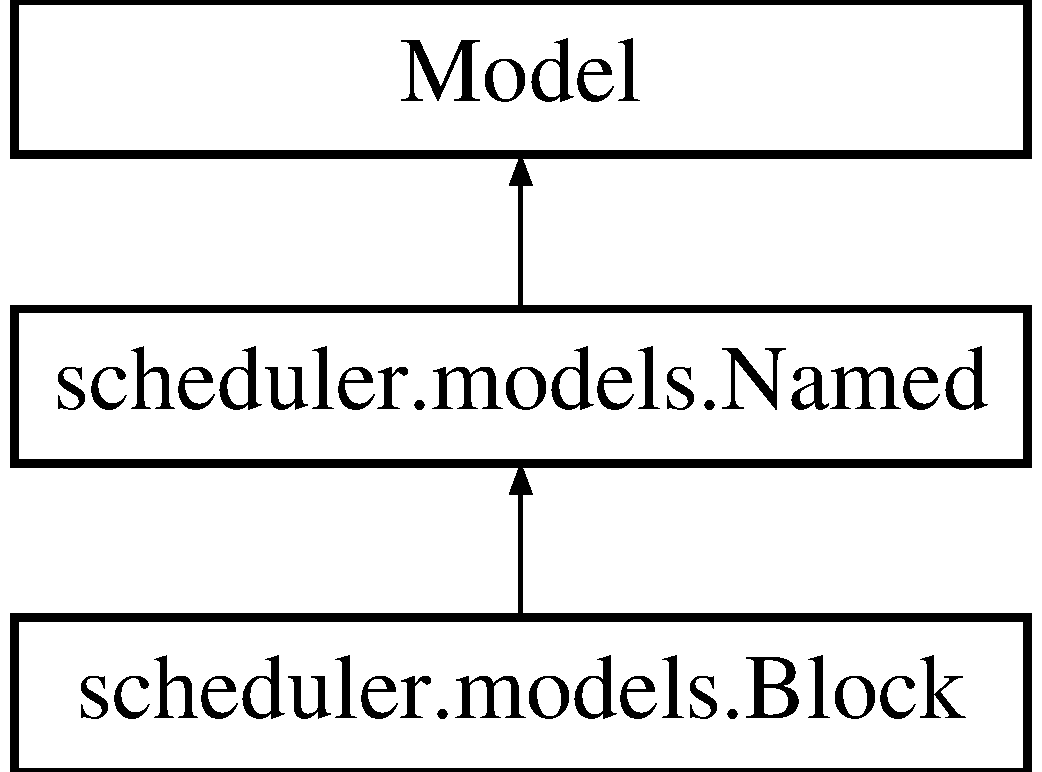
\includegraphics[height=3.000000cm]{classscheduler_1_1models_1_1_block}
\end{center}
\end{figure}
\subsection*{Static Public Attributes}
\begin{DoxyCompactItemize}
\item 
\hypertarget{classscheduler_1_1models_1_1_block_ab78204367b89bd16c9cb000d6bc8ecc6}{tuple {\bfseries next\-\_\-block} = models.\-One\-To\-One\-Field('self', on\-\_\-delete=models.\-C\-A\-S\-C\-A\-D\-E, related\-\_\-name=\char`\"{}previous\-\_\-block\char`\"{}, null=True, blank=True)}\label{classscheduler_1_1models_1_1_block_ab78204367b89bd16c9cb000d6bc8ecc6}

\item 
\hypertarget{classscheduler_1_1models_1_1_block_aa869281bbcdb191ddc5c0ed335e63109}{tuple {\bfseries paired\-\_\-with} = models.\-Foreign\-Key('self', on\-\_\-delete=models.\-C\-A\-S\-C\-A\-D\-E, related\-\_\-name=\char`\"{}paired\-\_\-with\-\_\-reverse\char`\"{}, null=True, blank=True)}\label{classscheduler_1_1models_1_1_block_aa869281bbcdb191ddc5c0ed335e63109}

\end{DoxyCompactItemize}
\subsection*{Additional Inherited Members}


The documentation for this class was generated from the following file\-:\begin{DoxyCompactItemize}
\item 
/home/travis/build/\-Open-\/\-Source-\/\-Software-\/\-Development/class-\/scheduler/mysite/scheduler/models.\-py\end{DoxyCompactItemize}

\hypertarget{classscheduler_1_1models_1_1_course}{\section{scheduler.\-models.\-Course Class Reference}
\label{classscheduler_1_1models_1_1_course}\index{scheduler.\-models.\-Course@{scheduler.\-models.\-Course}}
}
Inheritance diagram for scheduler.\-models.\-Course\-:\begin{figure}[H]
\begin{center}
\leavevmode
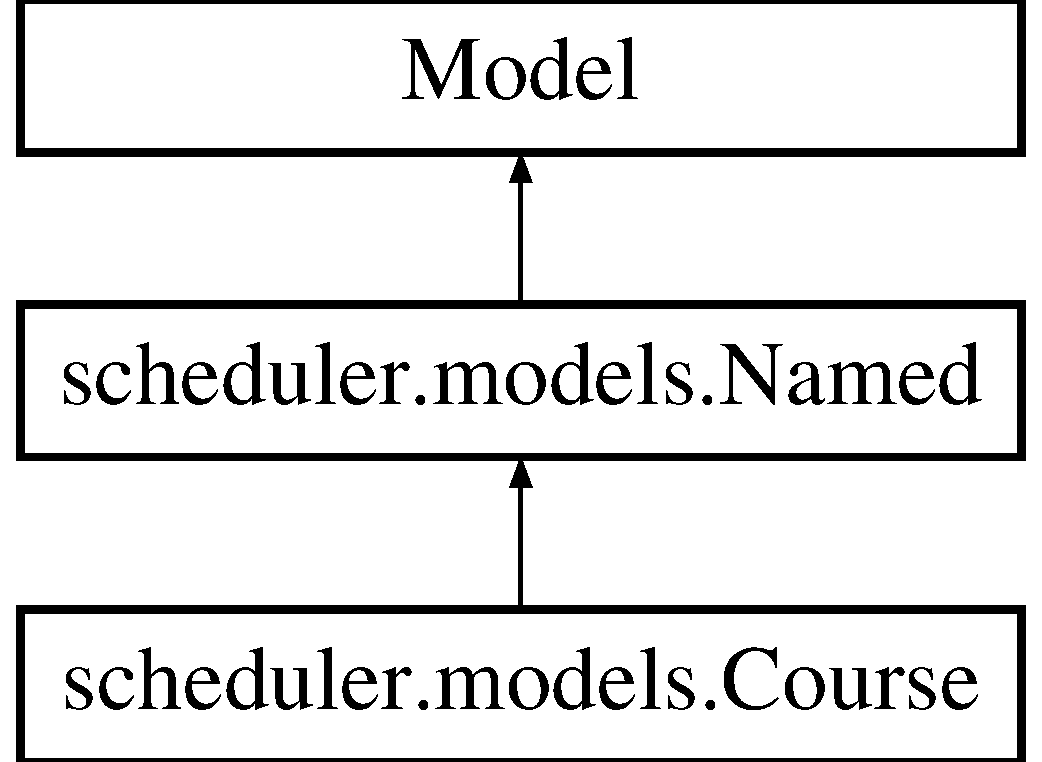
\includegraphics[height=3.000000cm]{classscheduler_1_1models_1_1_course}
\end{center}
\end{figure}
\subsection*{Static Public Attributes}
\begin{DoxyCompactItemize}
\item 
\hypertarget{classscheduler_1_1models_1_1_course_a469fbc25ba99da1185556bcd2d46f1b0}{tuple {\bfseries division} = models.\-Foreign\-Key(\hyperlink{classscheduler_1_1models_1_1_division}{Division}, on\-\_\-delete=models.\-C\-A\-S\-C\-A\-D\-E)}\label{classscheduler_1_1models_1_1_course_a469fbc25ba99da1185556bcd2d46f1b0}

\item 
\hypertarget{classscheduler_1_1models_1_1_course_a6a226c9c7cf238182071b5e00796af9a}{tuple {\bfseries program} = models.\-Char\-Field(max\-\_\-length=10)}\label{classscheduler_1_1models_1_1_course_a6a226c9c7cf238182071b5e00796af9a}

\item 
\hypertarget{classscheduler_1_1models_1_1_course_a1adc8da7f3f21d51f6262caea84123d7}{tuple {\bfseries title} = models.\-Char\-Field(max\-\_\-length=30, null=True, blank=True)}\label{classscheduler_1_1models_1_1_course_a1adc8da7f3f21d51f6262caea84123d7}

\item 
\hypertarget{classscheduler_1_1models_1_1_course_adcee98a824c0827372f76dd17d342409}{tuple {\bfseries ins\-\_\-method} = models.\-Char\-Field(max\-\_\-length=20, null=True, blank=True)}\label{classscheduler_1_1models_1_1_course_adcee98a824c0827372f76dd17d342409}

\item 
\hypertarget{classscheduler_1_1models_1_1_course_a8ea6f27aab56095042c8ef51b7715341}{tuple {\bfseries section\-\_\-capacity} = models.\-Positive\-Integer\-Field()}\label{classscheduler_1_1models_1_1_course_a8ea6f27aab56095042c8ef51b7715341}

\item 
\hypertarget{classscheduler_1_1models_1_1_course_a2d8ee964882dee311d4734297cb6c91b}{tuple {\bfseries style} = models.\-Char\-Field(max\-\_\-length=20, null=True, blank=True)}\label{classscheduler_1_1models_1_1_course_a2d8ee964882dee311d4734297cb6c91b}

\end{DoxyCompactItemize}
\subsection*{Additional Inherited Members}


\subsection{Detailed Description}
\begin{DoxyVerb}    Table: Course
    Primary Key: Composite (program, identifier)
    Columns:
        division: Foreign Key (Division)
            - The course's division code (ex: ITS)
        program: CharField (Max Length 10)
            -  The program identifier (ex: CSI)
        title: CharFierld (Max Length 30) 
            - The course title (ex: "intro to computer science" )
        section_capacity: Positive Integer
            - The maximum amout of registerable students in this course
            - Used to generate number of sections needed
        ins_method (instructional Method): CharField (Max Lenght 20)
            - The courses instructional method (ex STN)
        style: Charfield (Max Length 20)
            - The style of the course (ex: studio)\end{DoxyVerb}
 

The documentation for this class was generated from the following file\-:\begin{DoxyCompactItemize}
\item 
/home/travis/build/\-Open-\/\-Source-\/\-Software-\/\-Development/class-\/scheduler/mysite/scheduler/models.\-py\end{DoxyCompactItemize}

\hypertarget{classscheduler_1_1models_1_1_division}{\section{scheduler.\-models.\-Division Class Reference}
\label{classscheduler_1_1models_1_1_division}\index{scheduler.\-models.\-Division@{scheduler.\-models.\-Division}}
}
Inheritance diagram for scheduler.\-models.\-Division\-:\begin{figure}[H]
\begin{center}
\leavevmode
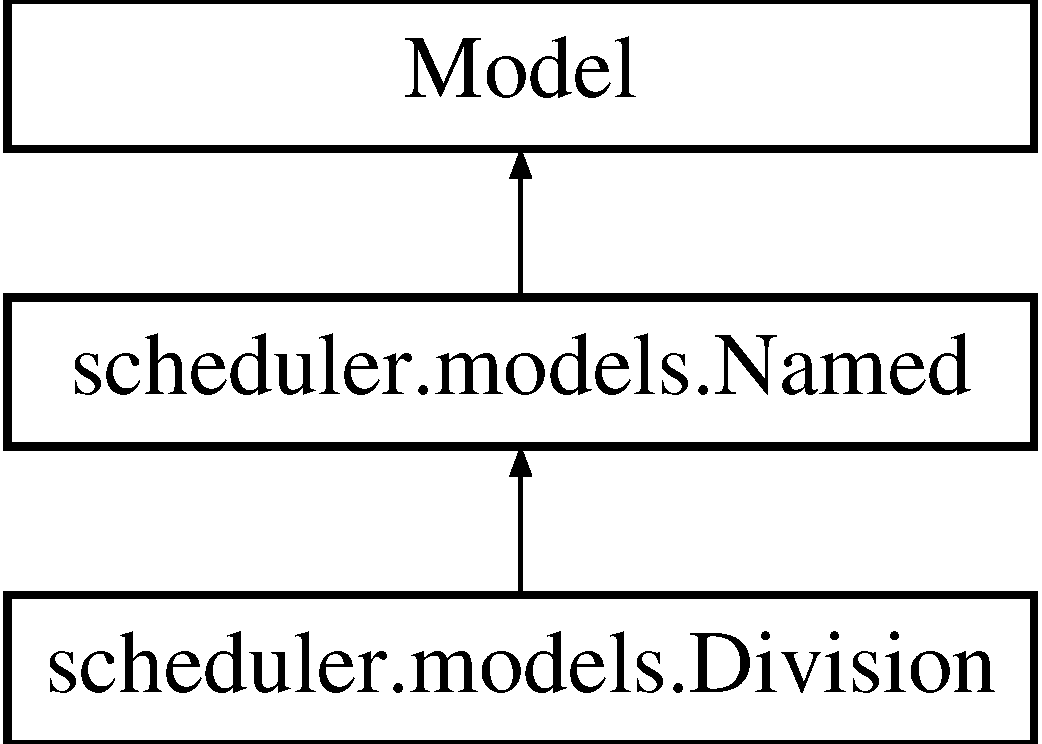
\includegraphics[height=3.000000cm]{classscheduler_1_1models_1_1_division}
\end{center}
\end{figure}
\subsection*{Additional Inherited Members}


\subsection{Detailed Description}
\begin{DoxyVerb}    Table: Division
    Primary Key: Autogenerated identifier.
    Columns: 
        division: CharField (Max Length: 20)
            - This should be all of the division identifiers (ex: ITS)
\end{DoxyVerb}
 

The documentation for this class was generated from the following file\-:\begin{DoxyCompactItemize}
\item 
/home/travis/build/\-Open-\/\-Source-\/\-Software-\/\-Development/class-\/scheduler/mysite/scheduler/models.\-py\end{DoxyCompactItemize}

\hypertarget{classscheduler_1_1models_1_1_hunk}{\section{scheduler.\-models.\-Hunk Class Reference}
\label{classscheduler_1_1models_1_1_hunk}\index{scheduler.\-models.\-Hunk@{scheduler.\-models.\-Hunk}}
}
Inheritance diagram for scheduler.\-models.\-Hunk\-:\begin{figure}[H]
\begin{center}
\leavevmode
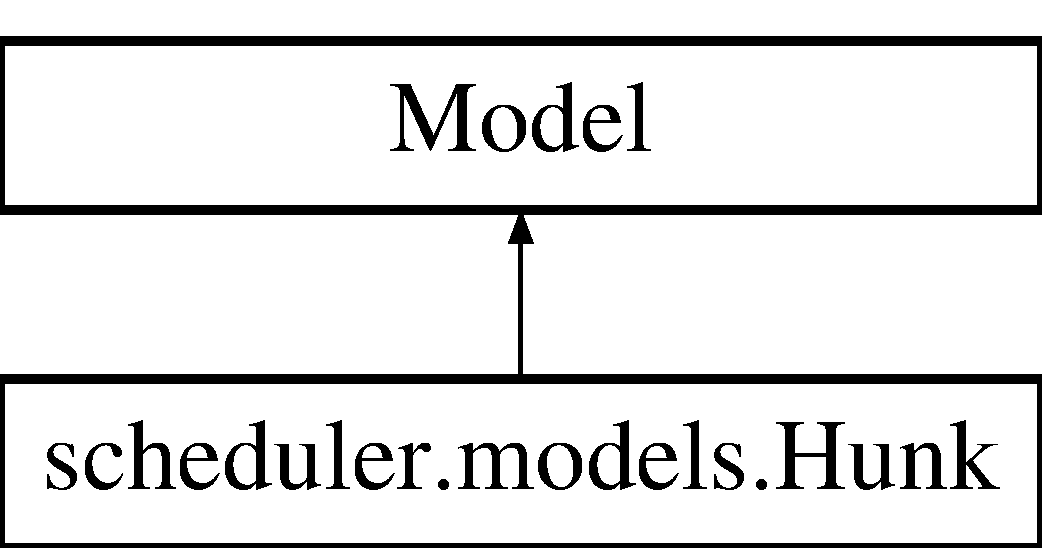
\includegraphics[height=2.000000cm]{classscheduler_1_1models_1_1_hunk}
\end{center}
\end{figure}
\subsection*{Public Member Functions}
\begin{DoxyCompactItemize}
\item 
\hypertarget{classscheduler_1_1models_1_1_hunk_a0ea2e3fef6321aa3e738390c537defde}{def {\bfseries \-\_\-\-\_\-str\-\_\-\-\_\-}}\label{classscheduler_1_1models_1_1_hunk_a0ea2e3fef6321aa3e738390c537defde}

\end{DoxyCompactItemize}
\subsection*{Static Public Attributes}
\begin{DoxyCompactItemize}
\item 
\hypertarget{classscheduler_1_1models_1_1_hunk_a24e5838d535817f4d0cb27f8fb6edd36}{tuple {\bfseries section} = models.\-Foreign\-Key(\hyperlink{classscheduler_1_1models_1_1_section}{Section}, on\-\_\-delete=models.\-C\-A\-S\-C\-A\-D\-E)}\label{classscheduler_1_1models_1_1_hunk_a24e5838d535817f4d0cb27f8fb6edd36}

\item 
\hypertarget{classscheduler_1_1models_1_1_hunk_aa01e29b62d649ce7cd0ccc0e35b51747}{tuple {\bfseries professor} = models.\-Foreign\-Key(\hyperlink{classscheduler_1_1models_1_1_professor}{Professor}, on\-\_\-delete=models.\-C\-A\-S\-C\-A\-D\-E)}\label{classscheduler_1_1models_1_1_hunk_aa01e29b62d649ce7cd0ccc0e35b51747}

\item 
\hypertarget{classscheduler_1_1models_1_1_hunk_ac50c8aaab3e58e9bf1ff953f4246f21a}{tuple {\bfseries room} = models.\-Foreign\-Key(\hyperlink{classscheduler_1_1models_1_1_room}{Room}, on\-\_\-delete=models.\-C\-A\-S\-C\-A\-D\-E)}\label{classscheduler_1_1models_1_1_hunk_ac50c8aaab3e58e9bf1ff953f4246f21a}

\item 
\hypertarget{classscheduler_1_1models_1_1_hunk_ab6e2df449de158fcf00218f6f2e63832}{tuple {\bfseries block} = models.\-Foreign\-Key(\hyperlink{classscheduler_1_1models_1_1_block}{Block}, on\-\_\-delete=models.\-C\-A\-S\-C\-A\-D\-E)}\label{classscheduler_1_1models_1_1_hunk_ab6e2df449de158fcf00218f6f2e63832}

\end{DoxyCompactItemize}


\subsection{Detailed Description}
\begin{DoxyVerb}    TODO:
        Documentation
\end{DoxyVerb}
 

The documentation for this class was generated from the following file\-:\begin{DoxyCompactItemize}
\item 
/home/travis/build/\-Open-\/\-Source-\/\-Software-\/\-Development/class-\/scheduler/mysite/scheduler/models.\-py\end{DoxyCompactItemize}

\hypertarget{classscheduler_1_1models_1_1_named_1_1_meta}{\section{scheduler.\-models.\-Named.\-Meta Class Reference}
\label{classscheduler_1_1models_1_1_named_1_1_meta}\index{scheduler.\-models.\-Named.\-Meta@{scheduler.\-models.\-Named.\-Meta}}
}
\subsection*{Static Public Attributes}
\begin{DoxyCompactItemize}
\item 
\hypertarget{classscheduler_1_1models_1_1_named_1_1_meta_a15a08f213947349b70c40da1a57d1e3c}{{\bfseries abstract} = True}\label{classscheduler_1_1models_1_1_named_1_1_meta_a15a08f213947349b70c40da1a57d1e3c}

\end{DoxyCompactItemize}


The documentation for this class was generated from the following file\-:\begin{DoxyCompactItemize}
\item 
/home/travis/build/\-Open-\/\-Source-\/\-Software-\/\-Development/class-\/scheduler/mysite/scheduler/models.\-py\end{DoxyCompactItemize}

\hypertarget{classscheduler_1_1models_1_1_user_preference_or_constraint_1_1_meta}{\section{scheduler.\-models.\-User\-Preference\-Or\-Constraint.\-Meta Class Reference}
\label{classscheduler_1_1models_1_1_user_preference_or_constraint_1_1_meta}\index{scheduler.\-models.\-User\-Preference\-Or\-Constraint.\-Meta@{scheduler.\-models.\-User\-Preference\-Or\-Constraint.\-Meta}}
}
\subsection*{Static Public Attributes}
\begin{DoxyCompactItemize}
\item 
\hypertarget{classscheduler_1_1models_1_1_user_preference_or_constraint_1_1_meta_a96e43107f2412f8afb1c0c2d416d151e}{{\bfseries abstract} = True}\label{classscheduler_1_1models_1_1_user_preference_or_constraint_1_1_meta_a96e43107f2412f8afb1c0c2d416d151e}

\end{DoxyCompactItemize}


The documentation for this class was generated from the following file\-:\begin{DoxyCompactItemize}
\item 
/home/travis/build/\-Open-\/\-Source-\/\-Software-\/\-Development/class-\/scheduler/mysite/scheduler/models.\-py\end{DoxyCompactItemize}

\hypertarget{classscheduler_1_1migrations_1_10001__initial_1_1_migration}{\section{scheduler.\-migrations.0001\-\_\-initial.Migration Class Reference}
\label{classscheduler_1_1migrations_1_10001__initial_1_1_migration}\index{scheduler.\-migrations.\-0001\-\_\-initial.\-Migration@{scheduler.\-migrations.\-0001\-\_\-initial.\-Migration}}
}
Inheritance diagram for scheduler.\-migrations.0001\-\_\-initial.Migration\-:\begin{figure}[H]
\begin{center}
\leavevmode
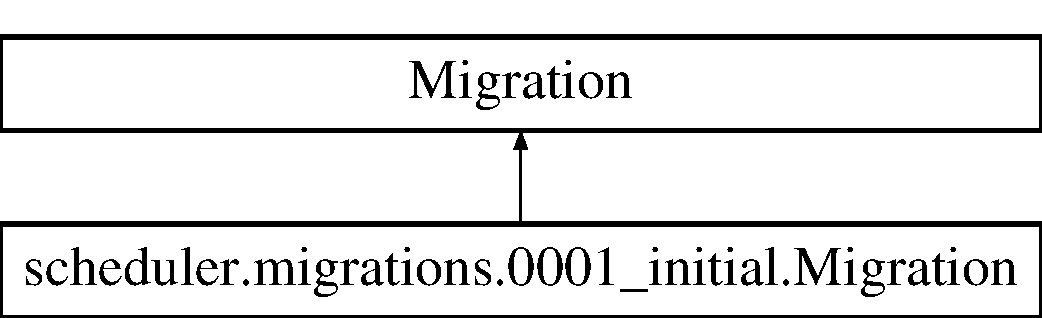
\includegraphics[height=2.000000cm]{classscheduler_1_1migrations_1_10001__initial_1_1_migration}
\end{center}
\end{figure}
\subsection*{Static Public Attributes}
\begin{DoxyCompactItemize}
\item 
\hypertarget{classscheduler_1_1migrations_1_10001__initial_1_1_migration_ae9fa974c12a7662b1a912aa3a1fcabc7}{{\bfseries initial} = True}\label{classscheduler_1_1migrations_1_10001__initial_1_1_migration_ae9fa974c12a7662b1a912aa3a1fcabc7}

\item 
list {\bfseries dependencies}
\item 
\hypertarget{classscheduler_1_1migrations_1_10001__initial_1_1_migration_a770d37ba1e0a9cb6ea5164be5c780e59}{list {\bfseries operations}}\label{classscheduler_1_1migrations_1_10001__initial_1_1_migration_a770d37ba1e0a9cb6ea5164be5c780e59}

\end{DoxyCompactItemize}


\subsection{Member Data Documentation}
\hypertarget{classscheduler_1_1migrations_1_10001__initial_1_1_migration_a832c1b4e3b6b97bcb86078337bc7d506}{\index{scheduler\-::migrations\-::0001\-\_\-initial\-::\-Migration@{scheduler\-::migrations\-::0001\-\_\-initial\-::\-Migration}!dependencies@{dependencies}}
\index{dependencies@{dependencies}!scheduler::migrations::0001_initial::Migration@{scheduler\-::migrations\-::0001\-\_\-initial\-::\-Migration}}
\subsubsection[{dependencies}]{\setlength{\rightskip}{0pt plus 5cm}list scheduler.\-migrations.\-0001\-\_\-initial.\-Migration.\-dependencies\hspace{0.3cm}{\ttfamily [static]}}}\label{classscheduler_1_1migrations_1_10001__initial_1_1_migration_a832c1b4e3b6b97bcb86078337bc7d506}
{\bfseries Initial value\-:}
\begin{DoxyCode}
1 = [
2         (\textcolor{stringliteral}{'contenttypes'}, \textcolor{stringliteral}{'0002\_remove\_content\_type\_name'}),
3     ]
\end{DoxyCode}


The documentation for this class was generated from the following file\-:\begin{DoxyCompactItemize}
\item 
/home/travis/build/\-Open-\/\-Source-\/\-Software-\/\-Development/class-\/scheduler/mysite/scheduler/migrations/0001\-\_\-initial.\-py\end{DoxyCompactItemize}

\hypertarget{classscheduler_1_1models_1_1_named}{\section{scheduler.\-models.\-Named Class Reference}
\label{classscheduler_1_1models_1_1_named}\index{scheduler.\-models.\-Named@{scheduler.\-models.\-Named}}
}
Inheritance diagram for scheduler.\-models.\-Named\-:\begin{figure}[H]
\begin{center}
\leavevmode
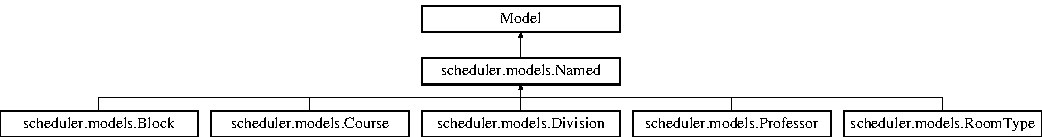
\includegraphics[height=1.846154cm]{classscheduler_1_1models_1_1_named}
\end{center}
\end{figure}
\subsection*{Classes}
\begin{DoxyCompactItemize}
\item 
class \hyperlink{classscheduler_1_1models_1_1_named_1_1_meta}{Meta}
\end{DoxyCompactItemize}
\subsection*{Public Member Functions}
\begin{DoxyCompactItemize}
\item 
\hypertarget{classscheduler_1_1models_1_1_named_a37b97c2fa4acbf5c61ca4cdff1410d47}{def {\bfseries \-\_\-\-\_\-str\-\_\-\-\_\-}}\label{classscheduler_1_1models_1_1_named_a37b97c2fa4acbf5c61ca4cdff1410d47}

\end{DoxyCompactItemize}
\subsection*{Static Public Attributes}
\begin{DoxyCompactItemize}
\item 
\hypertarget{classscheduler_1_1models_1_1_named_a5e5e18340ced82b633c6c913447d602f}{tuple {\bfseries name} = models.\-Char\-Field(max\-\_\-length=200, null=True)}\label{classscheduler_1_1models_1_1_named_a5e5e18340ced82b633c6c913447d602f}

\end{DoxyCompactItemize}


\subsection{Detailed Description}
\begin{DoxyVerb}    Gives better naming to things added manually
\end{DoxyVerb}
 

The documentation for this class was generated from the following file\-:\begin{DoxyCompactItemize}
\item 
/home/travis/build/\-Open-\/\-Source-\/\-Software-\/\-Development/class-\/scheduler/mysite/scheduler/models.\-py\end{DoxyCompactItemize}

\hypertarget{classscheduler_1_1models_1_1_pregen_section}{\section{scheduler.\-models.\-Pregen\-Section Class Reference}
\label{classscheduler_1_1models_1_1_pregen_section}\index{scheduler.\-models.\-Pregen\-Section@{scheduler.\-models.\-Pregen\-Section}}
}
Inheritance diagram for scheduler.\-models.\-Pregen\-Section\-:\begin{figure}[H]
\begin{center}
\leavevmode
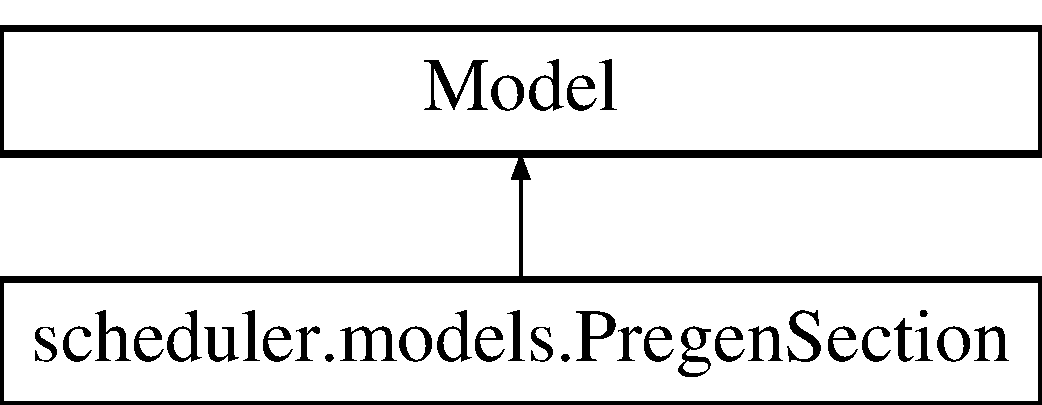
\includegraphics[height=2.000000cm]{classscheduler_1_1models_1_1_pregen_section}
\end{center}
\end{figure}
\subsection*{Public Member Functions}
\begin{DoxyCompactItemize}
\item 
\hypertarget{classscheduler_1_1models_1_1_pregen_section_a0f46c875c91c38646fdefea75fb5d652}{def {\bfseries \-\_\-\-\_\-str\-\_\-\-\_\-}}\label{classscheduler_1_1models_1_1_pregen_section_a0f46c875c91c38646fdefea75fb5d652}

\end{DoxyCompactItemize}
\subsection*{Static Public Attributes}
\begin{DoxyCompactItemize}
\item 
\hypertarget{classscheduler_1_1models_1_1_pregen_section_a3eafd0071b89cf3573c5f47c9194f848}{tuple {\bfseries course} = models.\-Foreign\-Key(\hyperlink{classscheduler_1_1models_1_1_course}{Course}, on\-\_\-delete=models.\-C\-A\-S\-C\-A\-D\-E)}\label{classscheduler_1_1models_1_1_pregen_section_a3eafd0071b89cf3573c5f47c9194f848}

\item 
\hypertarget{classscheduler_1_1models_1_1_pregen_section_ae51c6af4b08756b861dc5fe9bec2e203}{tuple {\bfseries suffix} = models.\-Char\-Field(max\-\_\-length=50)}\label{classscheduler_1_1models_1_1_pregen_section_ae51c6af4b08756b861dc5fe9bec2e203}

\end{DoxyCompactItemize}


\subsection{Detailed Description}
\begin{DoxyVerb}    TODO: Finish Table
    TODO: Documentation
\end{DoxyVerb}
 

The documentation for this class was generated from the following file\-:\begin{DoxyCompactItemize}
\item 
/home/travis/build/\-Open-\/\-Source-\/\-Software-\/\-Development/class-\/scheduler/mysite/scheduler/models.\-py\end{DoxyCompactItemize}

\hypertarget{classscheduler_1_1models_1_1_professor}{\section{scheduler.\-models.\-Professor Class Reference}
\label{classscheduler_1_1models_1_1_professor}\index{scheduler.\-models.\-Professor@{scheduler.\-models.\-Professor}}
}
Inheritance diagram for scheduler.\-models.\-Professor\-:\begin{figure}[H]
\begin{center}
\leavevmode
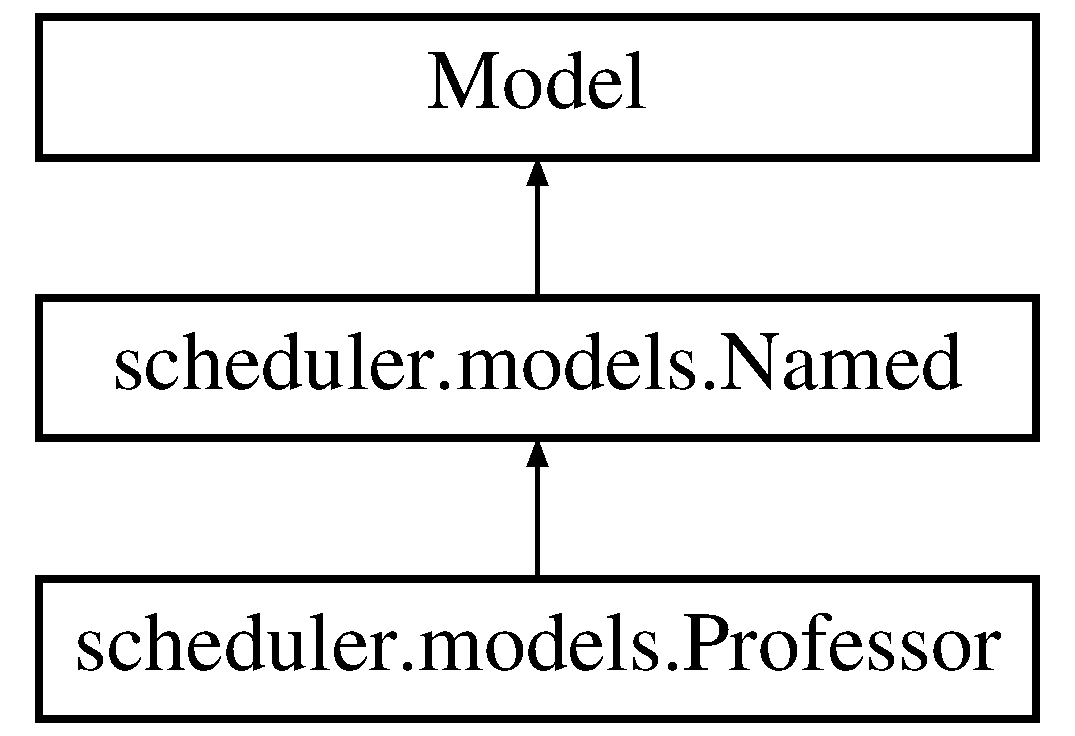
\includegraphics[height=3.000000cm]{classscheduler_1_1models_1_1_professor}
\end{center}
\end{figure}
\subsection*{Static Public Attributes}
\begin{DoxyCompactItemize}
\item 
\hypertarget{classscheduler_1_1models_1_1_professor_adf91e6bff4702170c31cb6135f23f31b}{tuple {\bfseries division} = models.\-Foreign\-Key(\hyperlink{classscheduler_1_1models_1_1_division}{Division}, on\-\_\-delete=models.\-C\-A\-S\-C\-A\-D\-E)}\label{classscheduler_1_1models_1_1_professor_adf91e6bff4702170c31cb6135f23f31b}

\item 
\hypertarget{classscheduler_1_1models_1_1_professor_a5a76821dd158b7ee380cac02a95ef14f}{tuple {\bfseries first} = models.\-Char\-Field(max\-\_\-length=20, null=True, blank=True)}\label{classscheduler_1_1models_1_1_professor_a5a76821dd158b7ee380cac02a95ef14f}

\item 
\hypertarget{classscheduler_1_1models_1_1_professor_a399cc5731fa62ed365a91c4c1dfe45d0}{tuple {\bfseries last} = models.\-Char\-Field(max\-\_\-length=20, null=True, blank=True)}\label{classscheduler_1_1models_1_1_professor_a399cc5731fa62ed365a91c4c1dfe45d0}

\item 
\hypertarget{classscheduler_1_1models_1_1_professor_a49cca96860ed2452e86fc3877ad9d767}{tuple {\bfseries qualifications} = models.\-Many\-To\-Many\-Field(\hyperlink{classscheduler_1_1models_1_1_course}{Course})}\label{classscheduler_1_1models_1_1_professor_a49cca96860ed2452e86fc3877ad9d767}

\end{DoxyCompactItemize}
\subsection*{Additional Inherited Members}


\subsection{Detailed Description}
\begin{DoxyVerb}    Table: Professor
    PrimaryKey: Autogenerated ID
    Columns:
        division: ForeignKey Division
        first: CharField(max_length=20)
            - Professors First Name (ex: James)
        last: CharField(max_length=20)
            -Professor Last Name (ex: Wilson)
        qualifications: ManyToManyField with Course
            -Each professor teaches multiple courses 
\end{DoxyVerb}
 

The documentation for this class was generated from the following file\-:\begin{DoxyCompactItemize}
\item 
/home/travis/build/\-Open-\/\-Source-\/\-Software-\/\-Development/class-\/scheduler/mysite/scheduler/models.\-py\end{DoxyCompactItemize}

\hypertarget{classscheduler_1_1models_1_1_room}{\section{scheduler.\-models.\-Room Class Reference}
\label{classscheduler_1_1models_1_1_room}\index{scheduler.\-models.\-Room@{scheduler.\-models.\-Room}}
}
Inheritance diagram for scheduler.\-models.\-Room\-:\begin{figure}[H]
\begin{center}
\leavevmode
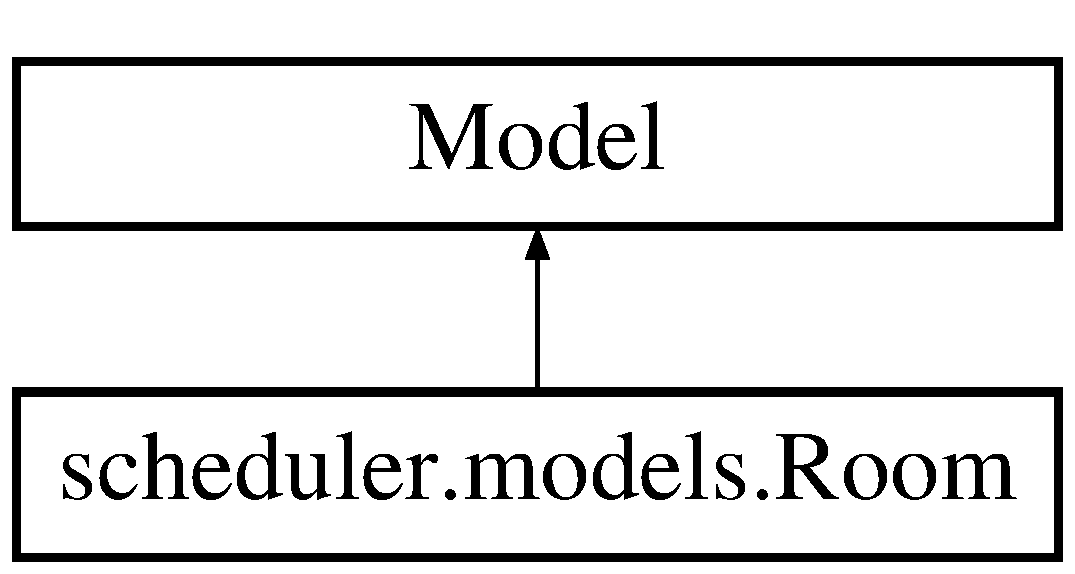
\includegraphics[height=3.000000cm]{classscheduler_1_1models_1_1_room}
\end{center}
\end{figure}
\subsection*{Static Public Attributes}
\begin{DoxyCompactItemize}
\item 
\hypertarget{classscheduler_1_1models_1_1_room_ae20a236603dca32bdaaad8e39c56f7ea}{tuple {\bfseries division} = models.\-Foreign\-Key(\hyperlink{classscheduler_1_1models_1_1_division}{Division}, on\-\_\-delete=models.\-C\-A\-S\-C\-A\-D\-E)}\label{classscheduler_1_1models_1_1_room_ae20a236603dca32bdaaad8e39c56f7ea}

\item 
\hypertarget{classscheduler_1_1models_1_1_room_ac160d40e28f0ce48c1b2843b225981ab}{tuple {\bfseries room\-\_\-type} = models.\-Foreign\-Key(\hyperlink{classscheduler_1_1models_1_1_room_type}{Room\-Type}, on\-\_\-delete=models.\-C\-A\-S\-C\-A\-D\-E)}\label{classscheduler_1_1models_1_1_room_ac160d40e28f0ce48c1b2843b225981ab}

\end{DoxyCompactItemize}
\subsection*{Additional Inherited Members}


The documentation for this class was generated from the following file\-:\begin{DoxyCompactItemize}
\item 
/home/travis/build/\-Open-\/\-Source-\/\-Software-\/\-Development/class-\/scheduler/mysite/scheduler/models.\-py\end{DoxyCompactItemize}

\hypertarget{classscheduler_1_1models_1_1_room_type}{\section{scheduler.\-models.\-Room\-Type Class Reference}
\label{classscheduler_1_1models_1_1_room_type}\index{scheduler.\-models.\-Room\-Type@{scheduler.\-models.\-Room\-Type}}
}
Inheritance diagram for scheduler.\-models.\-Room\-Type\-:\begin{figure}[H]
\begin{center}
\leavevmode
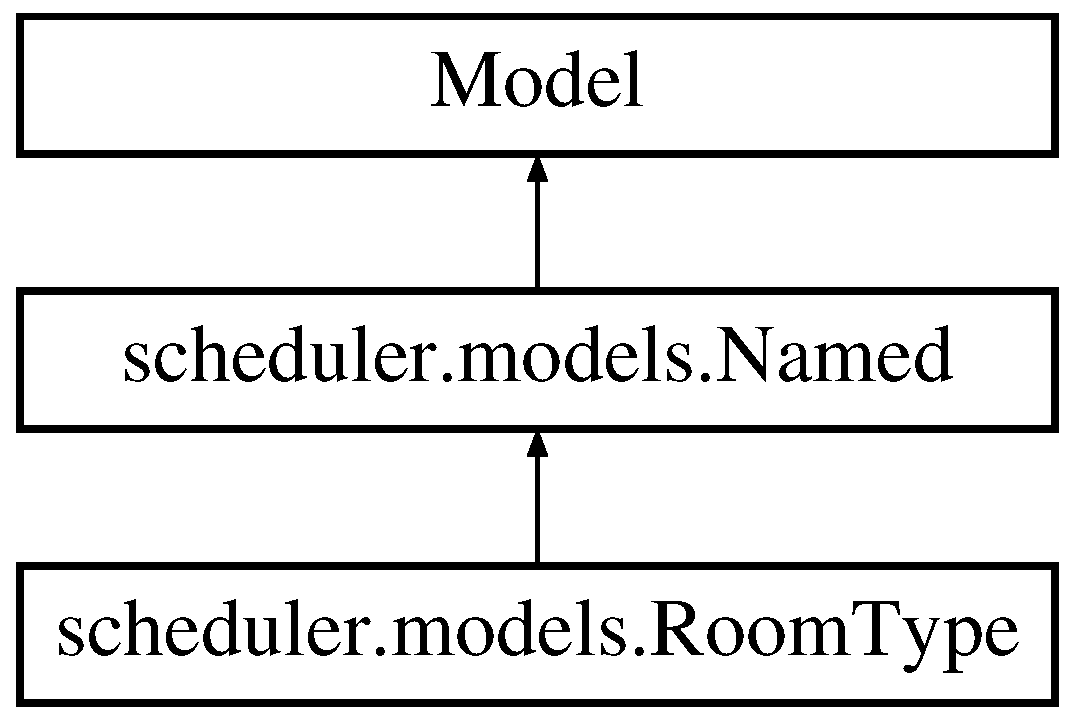
\includegraphics[height=3.000000cm]{classscheduler_1_1models_1_1_room_type}
\end{center}
\end{figure}
\subsection*{Additional Inherited Members}


The documentation for this class was generated from the following file\-:\begin{DoxyCompactItemize}
\item 
/home/travis/build/\-Open-\/\-Source-\/\-Software-\/\-Development/class-\/scheduler/mysite/scheduler/models.\-py\end{DoxyCompactItemize}

\hypertarget{classscheduler_1_1apps_1_1_scheduler_config}{\section{scheduler.\-apps.\-Scheduler\-Config Class Reference}
\label{classscheduler_1_1apps_1_1_scheduler_config}\index{scheduler.\-apps.\-Scheduler\-Config@{scheduler.\-apps.\-Scheduler\-Config}}
}
Inheritance diagram for scheduler.\-apps.\-Scheduler\-Config\-:\begin{figure}[H]
\begin{center}
\leavevmode
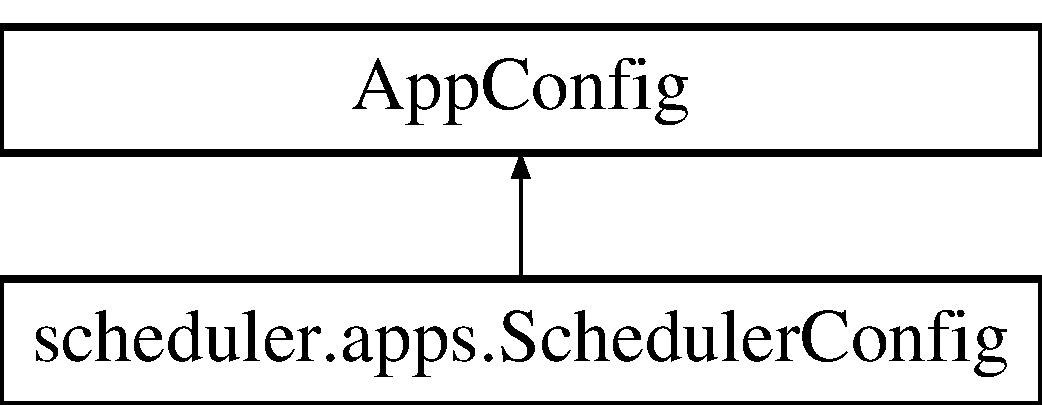
\includegraphics[height=2.000000cm]{classscheduler_1_1apps_1_1_scheduler_config}
\end{center}
\end{figure}
\subsection*{Static Public Attributes}
\begin{DoxyCompactItemize}
\item 
\hypertarget{classscheduler_1_1apps_1_1_scheduler_config_aebb64410f42031cde5364a964e8c85b3}{string {\bfseries name} = 'scheduler'}\label{classscheduler_1_1apps_1_1_scheduler_config_aebb64410f42031cde5364a964e8c85b3}

\end{DoxyCompactItemize}


The documentation for this class was generated from the following file\-:\begin{DoxyCompactItemize}
\item 
/home/travis/build/\-Open-\/\-Source-\/\-Software-\/\-Development/class-\/scheduler/mysite/scheduler/apps.\-py\end{DoxyCompactItemize}

\hypertarget{classscheduler_1_1models_1_1_section}{\section{scheduler.\-models.\-Section Class Reference}
\label{classscheduler_1_1models_1_1_section}\index{scheduler.\-models.\-Section@{scheduler.\-models.\-Section}}
}
Inheritance diagram for scheduler.\-models.\-Section\-:\begin{figure}[H]
\begin{center}
\leavevmode
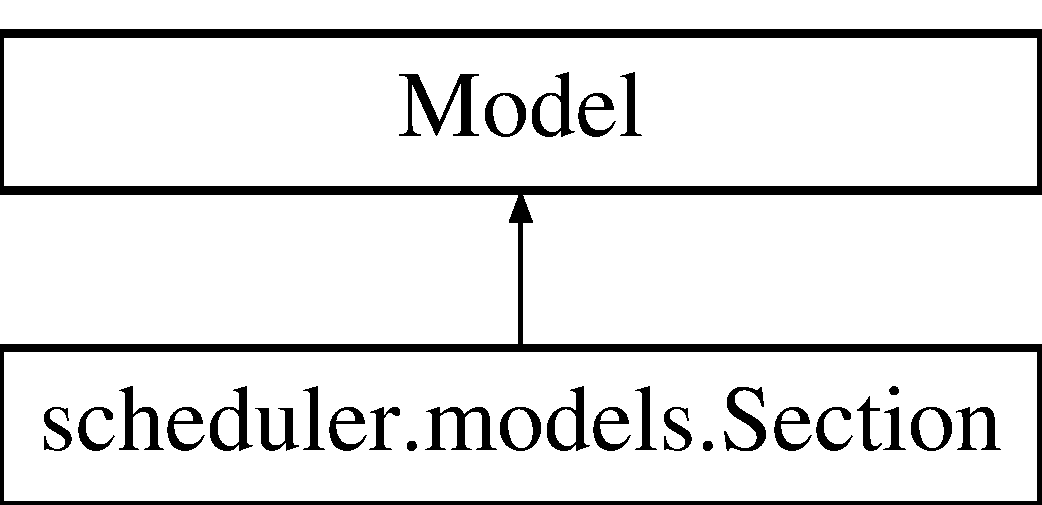
\includegraphics[height=2.000000cm]{classscheduler_1_1models_1_1_section}
\end{center}
\end{figure}
\subsection*{Public Member Functions}
\begin{DoxyCompactItemize}
\item 
\hypertarget{classscheduler_1_1models_1_1_section_a246a1f55dd3ce2f8b7e22b381535e09d}{def {\bfseries \-\_\-\-\_\-str\-\_\-\-\_\-}}\label{classscheduler_1_1models_1_1_section_a246a1f55dd3ce2f8b7e22b381535e09d}

\end{DoxyCompactItemize}
\subsection*{Static Public Attributes}
\begin{DoxyCompactItemize}
\item 
\hypertarget{classscheduler_1_1models_1_1_section_ac4fd835769f6add9617f8885b0d225fe}{tuple {\bfseries course} = models.\-Foreign\-Key(\hyperlink{classscheduler_1_1models_1_1_course}{Course}, on\-\_\-delete=models.\-C\-A\-S\-C\-A\-D\-E)}\label{classscheduler_1_1models_1_1_section_ac4fd835769f6add9617f8885b0d225fe}

\item 
\hypertarget{classscheduler_1_1models_1_1_section_a7cddf1d09f1567eb46674001375767b7}{tuple {\bfseries suffix} = models.\-Char\-Field(max\-\_\-length=50)}\label{classscheduler_1_1models_1_1_section_a7cddf1d09f1567eb46674001375767b7}

\end{DoxyCompactItemize}


The documentation for this class was generated from the following file\-:\begin{DoxyCompactItemize}
\item 
/home/travis/build/\-Open-\/\-Source-\/\-Software-\/\-Development/class-\/scheduler/mysite/scheduler/models.\-py\end{DoxyCompactItemize}

\hypertarget{classscheduler_1_1models_1_1_user_constaint}{\section{scheduler.\-models.\-User\-Constaint Class Reference}
\label{classscheduler_1_1models_1_1_user_constaint}\index{scheduler.\-models.\-User\-Constaint@{scheduler.\-models.\-User\-Constaint}}
}


T\-O\-D\-O\-: Documentation.  


Inheritance diagram for scheduler.\-models.\-User\-Constaint\-:\begin{figure}[H]
\begin{center}
\leavevmode
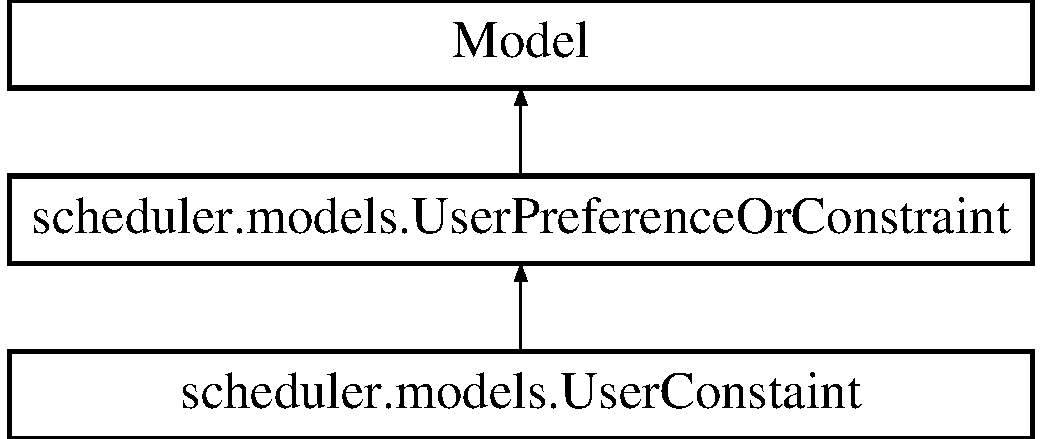
\includegraphics[height=3.000000cm]{classscheduler_1_1models_1_1_user_constaint}
\end{center}
\end{figure}
\subsection*{Public Member Functions}
\begin{DoxyCompactItemize}
\item 
\hypertarget{classscheduler_1_1models_1_1_user_constaint_a5a35e3eb2cd241453f4c1fbadb3c8812}{def \hyperlink{classscheduler_1_1models_1_1_user_constaint_a5a35e3eb2cd241453f4c1fbadb3c8812}{describe}}\label{classscheduler_1_1models_1_1_user_constaint_a5a35e3eb2cd241453f4c1fbadb3c8812}

\begin{DoxyCompactList}\small\item\em T\-O\-D\-O\-: Documentation. \end{DoxyCompactList}\end{DoxyCompactItemize}
\subsection*{Static Public Attributes}
\begin{DoxyCompactItemize}
\item 
\hypertarget{classscheduler_1_1models_1_1_user_constaint_a8817f2145d653131ad7084ad6ed71e97}{tuple \hyperlink{classscheduler_1_1models_1_1_user_constaint_a8817f2145d653131ad7084ad6ed71e97}{is\-\_\-blacklist} = models.\-Boolean\-Field()}\label{classscheduler_1_1models_1_1_user_constaint_a8817f2145d653131ad7084ad6ed71e97}

\begin{DoxyCompactList}\small\item\em T\-O\-D\-O\-: Documentation. \end{DoxyCompactList}\end{DoxyCompactItemize}


\subsection{Detailed Description}
T\-O\-D\-O\-: Documentation. 

The documentation for this class was generated from the following file\-:\begin{DoxyCompactItemize}
\item 
/home/travis/build/\-Open-\/\-Source-\/\-Software-\/\-Development/class-\/scheduler/mysite/scheduler/models.\-py\end{DoxyCompactItemize}

\hypertarget{classscheduler_1_1models_1_1_user_preference}{\section{scheduler.\-models.\-User\-Preference Class Reference}
\label{classscheduler_1_1models_1_1_user_preference}\index{scheduler.\-models.\-User\-Preference@{scheduler.\-models.\-User\-Preference}}
}


T\-O\-D\-O\-: Documentation.  


Inheritance diagram for scheduler.\-models.\-User\-Preference\-:\begin{figure}[H]
\begin{center}
\leavevmode
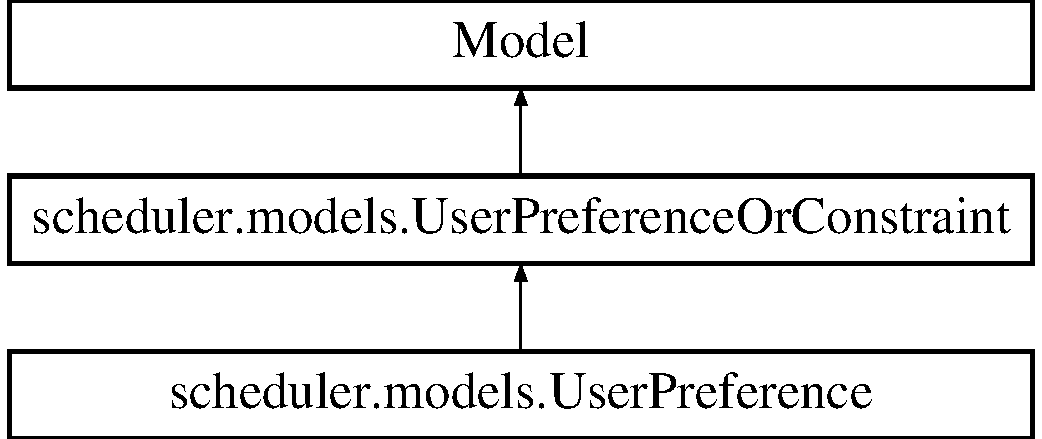
\includegraphics[height=3.000000cm]{classscheduler_1_1models_1_1_user_preference}
\end{center}
\end{figure}
\subsection*{Public Member Functions}
\begin{DoxyCompactItemize}
\item 
\hypertarget{classscheduler_1_1models_1_1_user_preference_a9f811ec38d568d99837e79b2b0699da6}{def \hyperlink{classscheduler_1_1models_1_1_user_preference_a9f811ec38d568d99837e79b2b0699da6}{describe}}\label{classscheduler_1_1models_1_1_user_preference_a9f811ec38d568d99837e79b2b0699da6}

\begin{DoxyCompactList}\small\item\em T\-O\-D\-O\-: Documentation. \end{DoxyCompactList}\end{DoxyCompactItemize}
\subsection*{Static Public Attributes}
\begin{DoxyCompactItemize}
\item 
\hypertarget{classscheduler_1_1models_1_1_user_preference_aefe583851d963dac6a85e6f8badfbffa}{tuple \hyperlink{classscheduler_1_1models_1_1_user_preference_aefe583851d963dac6a85e6f8badfbffa}{score} = models.\-Integer\-Field()}\label{classscheduler_1_1models_1_1_user_preference_aefe583851d963dac6a85e6f8badfbffa}

\begin{DoxyCompactList}\small\item\em T\-O\-D\-O\-: Documentation. \end{DoxyCompactList}\end{DoxyCompactItemize}


\subsection{Detailed Description}
T\-O\-D\-O\-: Documentation. 

The documentation for this class was generated from the following file\-:\begin{DoxyCompactItemize}
\item 
/home/travis/build/\-Open-\/\-Source-\/\-Software-\/\-Development/class-\/scheduler/mysite/scheduler/models.\-py\end{DoxyCompactItemize}

\hypertarget{classscheduler_1_1models_1_1_user_preference_or_constraint}{\section{scheduler.\-models.\-User\-Preference\-Or\-Constraint Class Reference}
\label{classscheduler_1_1models_1_1_user_preference_or_constraint}\index{scheduler.\-models.\-User\-Preference\-Or\-Constraint@{scheduler.\-models.\-User\-Preference\-Or\-Constraint}}
}


T\-O\-D\-O\-: Documentation.  


Inheritance diagram for scheduler.\-models.\-User\-Preference\-Or\-Constraint\-:\begin{figure}[H]
\begin{center}
\leavevmode
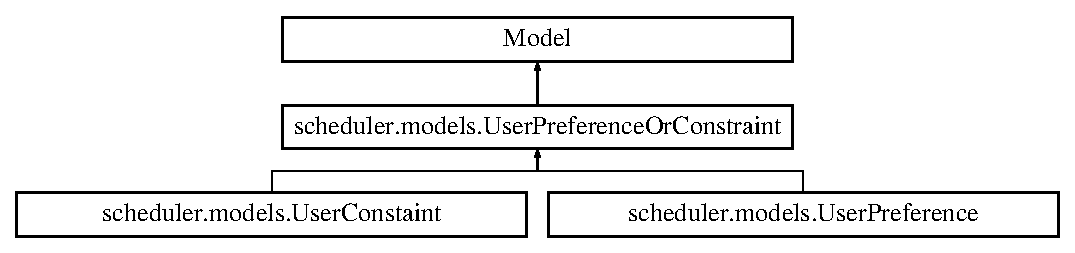
\includegraphics[height=2.947368cm]{classscheduler_1_1models_1_1_user_preference_or_constraint}
\end{center}
\end{figure}
\subsection*{Classes}
\begin{DoxyCompactItemize}
\item 
class \hyperlink{classscheduler_1_1models_1_1_user_preference_or_constraint_1_1_meta}{Meta}
\end{DoxyCompactItemize}
\subsection*{Public Member Functions}
\begin{DoxyCompactItemize}
\item 
\hypertarget{classscheduler_1_1models_1_1_user_preference_or_constraint_a1b04b83430b49ef79badd95682e6cf4e}{def \hyperlink{classscheduler_1_1models_1_1_user_preference_or_constraint_a1b04b83430b49ef79badd95682e6cf4e}{\-\_\-\-\_\-str\-\_\-\-\_\-}}\label{classscheduler_1_1models_1_1_user_preference_or_constraint_a1b04b83430b49ef79badd95682e6cf4e}

\begin{DoxyCompactList}\small\item\em T\-O\-D\-O\-: Documentation. \end{DoxyCompactList}\item 
\hypertarget{classscheduler_1_1models_1_1_user_preference_or_constraint_a8198615fa62dee4ea1cb89fe6ab834e0}{def \hyperlink{classscheduler_1_1models_1_1_user_preference_or_constraint_a8198615fa62dee4ea1cb89fe6ab834e0}{describe}}\label{classscheduler_1_1models_1_1_user_preference_or_constraint_a8198615fa62dee4ea1cb89fe6ab834e0}

\begin{DoxyCompactList}\small\item\em T\-O\-D\-O\-: Documentation. \end{DoxyCompactList}\end{DoxyCompactItemize}
\subsection*{Static Public Attributes}
\begin{DoxyCompactItemize}
\item 
\hypertarget{classscheduler_1_1models_1_1_user_preference_or_constraint_a0455877d277a31c0561935c7074b664b}{tuple \hyperlink{classscheduler_1_1models_1_1_user_preference_or_constraint_a0455877d277a31c0561935c7074b664b}{left\-\_\-argument\-\_\-type} = models.\-Foreign\-Key(Content\-Type, on\-\_\-delete=models.\-C\-A\-S\-C\-A\-D\-E, related\-\_\-name=\char`\"{}+\char`\"{})}\label{classscheduler_1_1models_1_1_user_preference_or_constraint_a0455877d277a31c0561935c7074b664b}

\begin{DoxyCompactList}\small\item\em T\-O\-D\-O\-: Documentation. \end{DoxyCompactList}\item 
\hypertarget{classscheduler_1_1models_1_1_user_preference_or_constraint_aa1b1f271f6f1f18d5e99996db4840337}{tuple \hyperlink{classscheduler_1_1models_1_1_user_preference_or_constraint_aa1b1f271f6f1f18d5e99996db4840337}{left\-\_\-argument\-\_\-id} = models.\-Positive\-Integer\-Field()}\label{classscheduler_1_1models_1_1_user_preference_or_constraint_aa1b1f271f6f1f18d5e99996db4840337}

\begin{DoxyCompactList}\small\item\em T\-O\-D\-O\-: Documentation. \end{DoxyCompactList}\item 
\hypertarget{classscheduler_1_1models_1_1_user_preference_or_constraint_a1880c90f057ecd54a9a484faa30e3df5}{tuple \hyperlink{classscheduler_1_1models_1_1_user_preference_or_constraint_a1880c90f057ecd54a9a484faa30e3df5}{left\-\_\-argument\-\_\-object} = Generic\-Foreign\-Key('\hyperlink{classscheduler_1_1models_1_1_user_preference_or_constraint_a0455877d277a31c0561935c7074b664b}{left\-\_\-argument\-\_\-type}', '\hyperlink{classscheduler_1_1models_1_1_user_preference_or_constraint_aa1b1f271f6f1f18d5e99996db4840337}{left\-\_\-argument\-\_\-id}')}\label{classscheduler_1_1models_1_1_user_preference_or_constraint_a1880c90f057ecd54a9a484faa30e3df5}

\begin{DoxyCompactList}\small\item\em T\-O\-D\-O\-: Documentation. \end{DoxyCompactList}\item 
\hypertarget{classscheduler_1_1models_1_1_user_preference_or_constraint_a30dcc18f79528b7860691bced63d3426}{tuple \hyperlink{classscheduler_1_1models_1_1_user_preference_or_constraint_a30dcc18f79528b7860691bced63d3426}{right\-\_\-argument\-\_\-type} = models.\-Foreign\-Key(Content\-Type, on\-\_\-delete=models.\-C\-A\-S\-C\-A\-D\-E, related\-\_\-name=\char`\"{}+\char`\"{})}\label{classscheduler_1_1models_1_1_user_preference_or_constraint_a30dcc18f79528b7860691bced63d3426}

\begin{DoxyCompactList}\small\item\em T\-O\-D\-O\-: Documentation. \end{DoxyCompactList}\item 
\hypertarget{classscheduler_1_1models_1_1_user_preference_or_constraint_adbb69d170fd984fe2ec36e340cdf3533}{tuple \hyperlink{classscheduler_1_1models_1_1_user_preference_or_constraint_adbb69d170fd984fe2ec36e340cdf3533}{right\-\_\-argument\-\_\-id} = models.\-Positive\-Integer\-Field()}\label{classscheduler_1_1models_1_1_user_preference_or_constraint_adbb69d170fd984fe2ec36e340cdf3533}

\begin{DoxyCompactList}\small\item\em T\-O\-D\-O\-: Documentation. \end{DoxyCompactList}\item 
\hypertarget{classscheduler_1_1models_1_1_user_preference_or_constraint_a3a80b4294939af457c24a9377bc43239}{tuple \hyperlink{classscheduler_1_1models_1_1_user_preference_or_constraint_a3a80b4294939af457c24a9377bc43239}{right\-\_\-argument\-\_\-object} = Generic\-Foreign\-Key('\hyperlink{classscheduler_1_1models_1_1_user_preference_or_constraint_a30dcc18f79528b7860691bced63d3426}{right\-\_\-argument\-\_\-type}', '\hyperlink{classscheduler_1_1models_1_1_user_preference_or_constraint_adbb69d170fd984fe2ec36e340cdf3533}{right\-\_\-argument\-\_\-id}')}\label{classscheduler_1_1models_1_1_user_preference_or_constraint_a3a80b4294939af457c24a9377bc43239}

\begin{DoxyCompactList}\small\item\em T\-O\-D\-O\-: Documentation. \end{DoxyCompactList}\end{DoxyCompactItemize}


\subsection{Detailed Description}
T\-O\-D\-O\-: Documentation. 

The documentation for this class was generated from the following file\-:\begin{DoxyCompactItemize}
\item 
/home/travis/build/\-Open-\/\-Source-\/\-Software-\/\-Development/class-\/scheduler/mysite/scheduler/models.\-py\end{DoxyCompactItemize}

%--- End generated contents ---

% Index
\newpage
\phantomsection
\addcontentsline{toc}{chapter}{Index}
\printindex

\end{document}
